\chapter{مفاهیم اولیه‌}\label{chapter2}

در این بخش به توضیح بیشتر مفاهیم معرفی شده (اینترنت اشیاء، رایانش ابری و بدون سرور) پرداخته شده، سپس پروژه‌ها و راه حل های موجود برای توسعه هر کدام از این محیط‌ها بررسی می‌شود.

\section{اینترنت اشیاء}

 هم اکنون در ایران حدود ۱۵۰ شرکت خصوصی در حوزه اینترنت اشیاء فعال هستند که ۵۰ درصد در ارائه سرویس‌های نرم‌افزاری و برنامه‌های کاربردی، ۴۲ درصد در بخش سخت‌افزار و حسگرها و باقی در بخش بسترها و امنیت فعالیت می‌کنند.
% \cite{https://www.ovio.ir/2580/اینترنت-اشیا-در-ایران/}

\section{کانتینرها و هماهنگ کننده‌ی کانتینری}

\subsection{کانتیرها}

کانتینرها اجازه بسته‌بندی برنامه‌های کاربردی را به همراه تمام قسمت‌هایی که نیاز دارند شامل کتابخانه‌ها و دیگر وابستگی‌هایش، به توسعه‌دهنده‌ها می‌دهند. به زبان دیگر می‌توانیم کانتینر را شامل پردازه در حال اجرا و منابع سخت‌افزاری اختصاص داده شده به آن پردازه تعریف کرد.(شکل
\ref{تصویر 2-1}
) پس کانتینر به معنی یک قسمت سخت‌افزاری و قابل رویت نیست بلکه یک تعریف انتزاعی به معنای یک پردازه یا گروهی از پردازه‌ها به همراه منابع تخصیص داده شده به آن‌ها می‌باشد. 

\begin{figure}[!h]
	\centering
	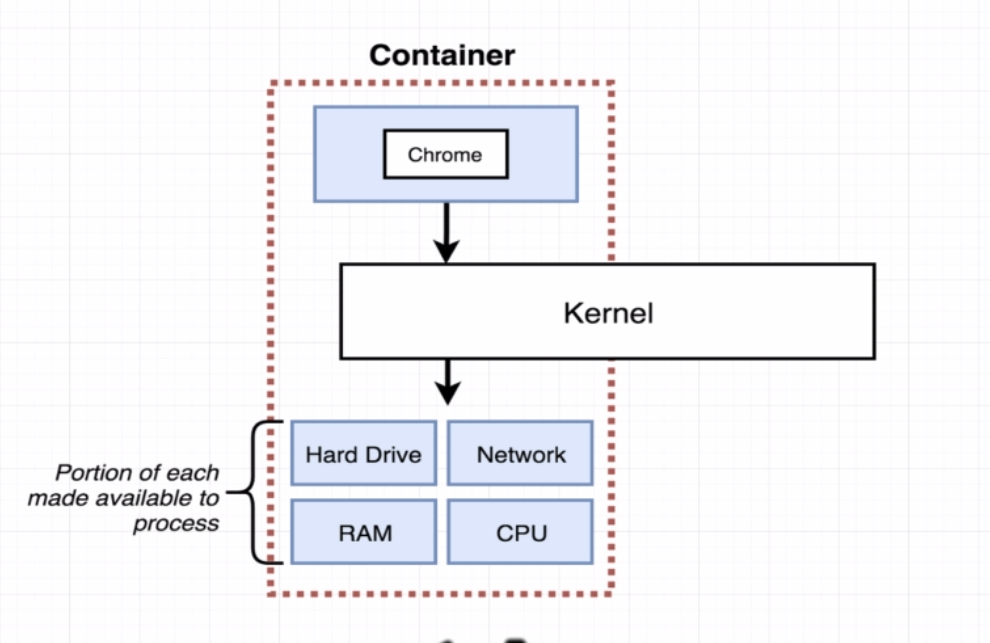
\includegraphics[height=6cm]{fig2-1}
	\caption{نمایش یک کانتینر}
	\label{تصویر 2-1}
\end{figure}

کانتینرها مکانیزم منطقی بسته‌بندی ارائه می‌دهند بدین معنا که برنامه‌های کاربردی می‌توانند از محیطی که در آن در حال اجرا هستند جدا شوند. این جداسازی باعث می‌شود تا برنامه‌های کاربردی مبتنی بر کانتینرها به راحتی و بدون درنظر گرفتن محیط هدف مستقر شوند. کانتینرایز کردن برنامه‌ها منجربه آن می‌شود که توسعه‌دهندگان تنها بر منطق برنامه فکر کنند و تیم‌های عملیات تکنولوژی اطلاعات بر روی استقرار و مدیریت آن تمرکز کنند.

برای کسانی که با محیط‌های مجازی‌سازی شده کار کرده‌اند، کانتینرها معمولاً با ماشین‌های مجازی مقایسه می‌شوند. ماشین مجازی به صورت یک سیستم عامل میهمان بر روی یک سیستم عامل میزبان با دسترسی‌های مجازی‌سازی‌شده به سخت‌افزار می‌باشد. همانند ماشین‌های مجازی، کانتینرها به شما این امکان را می‌دهند که برنامه خود را با تمام کتابخانه‌ها و وابستگی‌هایش بسته‌بندی کنید. این کار یک محیط مستقل و ایزوله برای اجرای سرویس‌های نرم‌افزاری را در اختیار شما قرار می‌دهد. 

برخلاف یک ماشین مجازی، یک کانتینر دارای یک سیستم عامل مجزا نمی‌باشد. سیستم عامل‌ها
\lr{kernel}
دارند که یک پروسه اجرایی نرم‌افزاری\LTRfootnote{running software process} می‌باشد و وظیفه آن کنترل دسترسی بین برنامه‌های در حال اجرا به منابع سخت‌افزاری موجود در کامپیوتر است.

سیستم عامل‌ها ویژگی به نام
\lr{name spacing}
دارند که به وسیله آن می‌شود قطعه‌هایی\LTRfootnote{segments} از منابع سخت‌افزاری موجود ساخت و آنها را به یک برنامه خاص اختصاص داد. در نتیجه به وسیله
\lr{name spacing}
می‌شود منبع سخت‌افزاری را بر طبق  پردازه یا برنامه اجرایی جدا و ایزوله کرد. البته ویژگی
\lr{name spacing}
فقط برای سخت‌افزار نمی‌باشد و برای نرم‌افزار هم تعریف می‌شود. یک ویژگی دیگر هم با نام
\lr{control group}
وجود دارد که به وسیله آن می‌توان مقدار منبعی که یک پردازه می‌تواند استفاده کند را محدود کرد. در نتیجه به وسیله این دو ویژگی می‌توان برای هر پردازه منابعی را اختصاص داد و آن منابع را محدود کرد. 

در این میان نیاز به تعریف مفهومی با عنوان ایمیج\LTRfootnote{image}داریم. ایمیج فایل‌های سیستمی\LTRfootnote{file system} است که شامل همه‌ی وابستگی‌ها و تنظیمات موردنیاز برای اجرای یک برنامه خاص می‌باشد. ایمیج را می‌توان به کانتینر تبدیل کرد. برای این کار ابتدا
\lr{kernel}
منابع سخت‌افزاری لازم را جدا می‌کند به طوری که فقط پردازه‌های کانتینر موردنظر می‌توانند به این منابع دسترسی داشته باشند. در ادامه فایل‌های موردنیاز آن کانتینر نیز جدا می‌شوند و بدین ترتیب یک کانتینر ساخته می‌شود.


\subsection{داکر}

در قسمت قبل با مفهوم کانتینر آشنا شدیم. حال سوال این است که چگونه می‌توانیم کانتینر را بسازیم و سپس با آن کار کنیم؟ در این قسمت با ابزاری به نام داکر آشنا می‌شویم.

\subsubsection{مفاهیم اولیه}

داکر یک پلتفرم کانتینرسازی (کانتینرکننده) است که برنامه کاربردی شما را با تمام وابستگی‌هایش در داخل یک کانتینر داکر بسته‌بندی (پکیج‌بندی) می‌کند و این اطمینان را به شما می‌دهد که برنامه شما در هر محیطی کار می‌کند.

حال سؤال این است که این بسته‌بندی استاندارد چه مزایایی دارد؟ این سؤال را می‌توان با یک مثال ساده پاسخ داد: فرض کنید یک شرکت می‌خواهد یک برنامه کاربردی وب با زبان برنامه‌نویسی جاوااسکریپت و فریمورک
\lr{react js}
را توسعه دهد. در نتیجه یک توسعه‌دهنده استخدام می‌کند که که این کار را انجام دهد. توسعه‌دهنده برنامه‌های مورد نیاز برای اجرای یک پروژه مانند
\lr{node js}
و پکیج منیجر\LTRfootnote{package manager}
\lr{npm}
را در سیستم خود نصب می‌کند و کار خود را شروع می‌کند. زمانی که توسعه دادن محصول به پایان رسید، توسعه‌دهنده محصول را جهت تست به تست‌کننده‌ی\LTRfootnote{tester} شرکت می‌دهد. تست‌کننده نیز لازم دارد برنامه‌های مورد نیاز جهت اجرای پروژه را بر روی سیستم خود نصب کند. همچنین بعد از تست محصول باید بر روی سرور قرار بگیرد در نتیجه بار دیگر لازم است این برنامه‌های راه‌انداز محصول بر روی سرور به صورت دستی نصب شود و خلاصه در هر سیستمی که می‌خواهید این محصول را اجرا کنید باید چندین برنامه نصب کنید. با توجه به این مثال به طور کلی به این مشکل پی می‌بریم که با توجه به گسترش ابزارهای نرم‌افزاری یه استاندارد کلی برای برنامه‌های نرم‌افزاری موجود نمی‌باشد و برنامه‌های نرم‌افزاری از نظر نحوه اجرا بسیار متفاوت‌اند.  برای جلوگیری از این مشکلات راه حل داکر بسیار مفید است. توسعه‌دهنده برای محصول خود یک ایمیج داکر ایجاد می‌کند و هر کس که می‌خواهد برنامه کاربردی را اجرا کند تنها کافی است ایمیج داکر را گرفته و با ابزار داکر که بر روی سیستم خود نصب کرده است آن را بر روی سیستم خود اجرا کند.

برای کسانی که با ماشین‌های مجازی آشنا هستند این ابهام پیش می‌آید که این کار را ماشین‌های مجازی نیز انجام می‌دهند.  می‌توان در سه پارامتر اساسی کانتینر داکر و ماشین مجازی را با یکدگیر مقایسه کرد:
\cite{Edureka_DiveIntoDocker}

\begin{enumerate}
	\item 
	سایز: منابعی که هر کدام استفاده می‌کنند
	\item 
	زمان راه‌اندازی\LTRfootnote{startup} : زمان
	\lr{boot}
	سیستم 
	\item 
	ادغام\LTRfootnote{integration} : قابلیت ادغام با ابزارهای دیگر
\end{enumerate}

\subsubsection*{سایز}


\begin{figure}[!h]
	\centering
	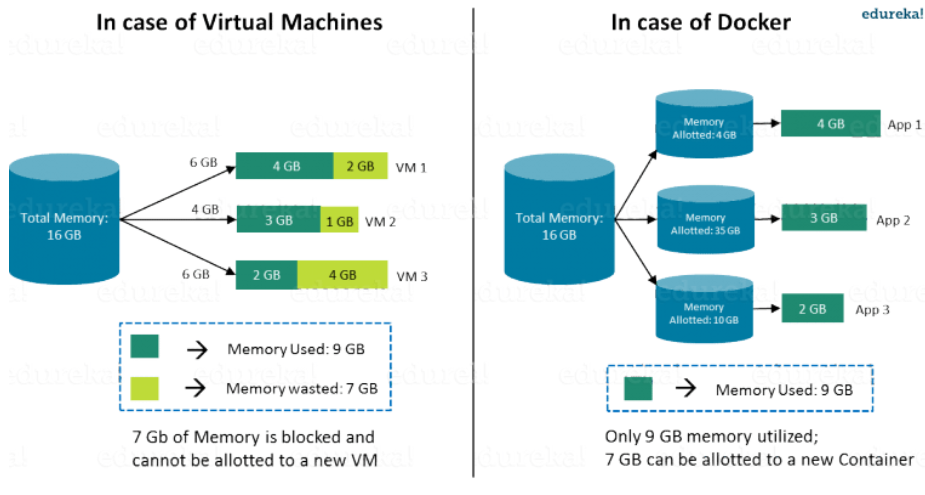
\includegraphics[width=\linewidth]{fig2-2}
	\caption{مقایسه سایز نمونه‌ها در محیط کانتینری و محیط مجازی}
	\label{تصویر 2-2}
\end{figure}

وقتی از ماشین‌های مجازی استفاده می‌کنید، به صورت موازی باید حافظه رم را بین ماشین مجازی ایجاد شده تقسیم کرد. در این حالت ممکن است ماشین مجازی ما کمتر از مقدار اختصاص داده شده به آن حافظه مصرف کند. در نتیجه مقداری از حافظه رم بلاک می‌شود و بدون مصرف باقی می‌ماند و همچنین نمی‌توان آن را به ماشین مجازی دیگری اختصاص داد زیرا قبلاً تخصیص داده شده‌است. در حالی که اگر از کانتینر استفاده شود،
\lr{cpu}
دقیقاً به اندازه مقدار حافظه‌ای که کانتینر نیاز دارد به آن حافظه اختصاص می‌دهد. درنتیجه از هدر دادن حافظه رم جلوگیری می‌شود و می‌توان تعداد کانتینرهای بیشتری را به صورت موازی اجرا کرد. (‌شکل 
\ref{تصویر 2-2}
)

\subsubsection*{زمان راه‌اندازی}

\begin{figure}[!h]
	\centering
	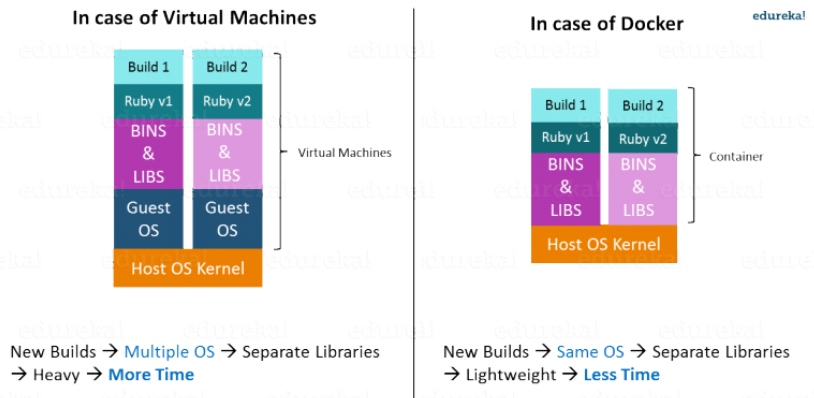
\includegraphics[height=6cm]{fig2-3}
	\caption{مقایسه زمان راه‌اندازی نمونه‌ها در محیط کانتینری و محیط مجازی}
	\label{تصویر 2-3}
\end{figure}

وقتی یک ماشین مجازی می‌خواهد راه‌اندازی شود، زمان زیادی لازم است تا سیستم عامل مهمان از ابتدا راه‌اندازی شود و سپس تمام فایل‌ها و کتاب‌خانه‌های آن بارگذاری شوند. این در حالی است که اگر از کانتینر داکر استفاده شود، این زمان راه‌اندازی سیستم عامل مهمان دیگر وجود ندارد. (شکل
\ref{تصویر 2-3}
)

\subsubsection*{قابلیت ادغام}

\begin{figure}[!h]
	\centering
	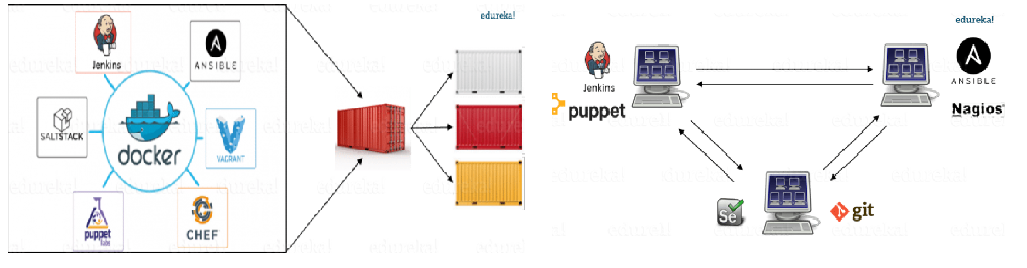
\includegraphics[height=3.5cm]{fig2-4}
	\caption{مقایسه قابلیت ادغام نمونه‌ها در محیط کانتینری و محیط مجازی}
	\label{تصویر 2-4}
\end{figure}

ادغام ابزارهای مختلف به وسیله ماشین‌های مجازی شاید کار ممکنی باشد اما همراه با پیچیدگی‌های بسیاری می‌باشد. اگر نیاز دارید چندین نمونه از یک یا چند ابزار نرم‌افزاری را با استفاده از ماشین‌های مجازی راه‌اندازی و استفاده کنید، باید مدام ابزارهای خود را بین ماشین‌ها بچرخانید زیرا هر ماشین تنها قادر به اجرای یک نمونه از یک ابزار می‌باشد. در حالی که با استفاده کانتینرهای داکر می‌توانید چندین نمونه از چندین ابزار را در یک یا چند کانتینر همزمان اجرا کنید و همچنین با کپی‌کردن کانتینرها می‌توانید مقیاس‌بندی لازم را انجام دهید. ( شکل 
\ref{تصویر 2-4}
)


\subsubsection{تعاریف مورداستفاده}

پس از آشنایی با ابزار داکر و قابلیت‌های آن و مقایسه عملکرد آن با ماشین‌های مجازی، در این قسمت به معرفی تعاریف تخصصی‌تری می‌پردازیم. شناخت این مفاهیم جهت کار کردن در محیط داکری لازم و ضروری است.

\subsubsection*{داکر اینجین}
داکر اینجین\LTRfootnote{docker engine} به عنوان قلب یک سیستم داکری شناخته می‌شود. یک تکنولوژی قدرتمند و سبک وزن کانترایز کردن \LTRfootnote{containerization} می‌باشد که وظیفه‌ی ساخت و کانتینر کردن برنامه‌های کاربردی را بر عهده دارد. این تکنولوژی بر روی ماشین میزبان نصب می‌شود و همانند یک برنامه مشتری-سرویس‌دهنده\LTRfootnote{client-server} عمل می‌کند. بدین منظور از ابزارهای زیر استفاده می‌کند:
\begin{enumerate}
	\item 
	یک سرور از نوع برنامه طولانی مدت \LTRfootnote{long-running program} که
	\lr{daemon process}
	نامیده می‌شود.
	\item 
	یک رابط خط فرمان\LTRfootnote{CLI} به عنوان مشتری\LTRfootnote{client}
	
	\item 
	\lr{REST API}
	جهت ارتباط بین
	\lr{CLI client}
	و
	\lr{Docker Daemon}
	
\end{enumerate}

\begin{figure}[!h]
	\centering
	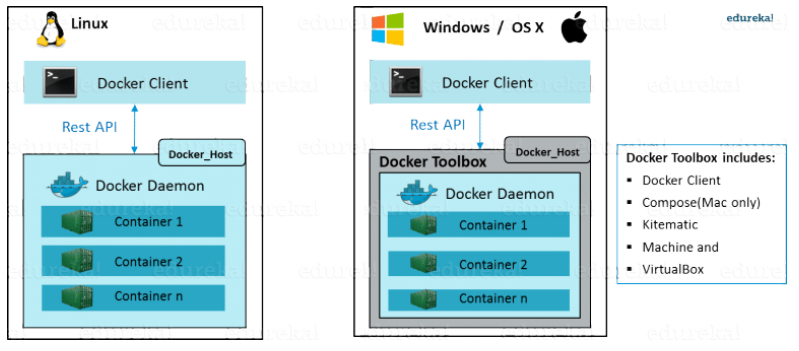
\includegraphics[height=5cm]{fig2-5}
	\caption{ساختار داکر اینجین}
	\label{تصویر 2-5}
\end{figure}

همان‌طور که در تصویر (شکل 
\ref{تصویر 2-5}
) دیده می‌شود به عنوان نمونه در سیستم عامل
\lr{linux}
،
\lr{Docker client}
از طریق ترمینال در دسترس است و
\lr{Docker Daemon}
بر روی
\lr{Docker Host}
اجرا می‌شود. 


\subsubsection*{داکر ایمیج}
داکر ایمیج \LTRfootnote{Docker Image} یک فایل است که از چندین لایه تشکیل شده است و برای اجرا کردن کد در کانتینر داکر استفاده می‌شود. اساسا ایمیج از دستورالعمل‌هایی برای قابل اجرا کردن برنامه کاربردی ساخته می‌شود و جهت اجرا بر روی 
\lr{kernel}
های سیستم عامل قرار می‌گیرد. وقتی کاربر یک ایمیج را اجرا می‌کند، این ایمیج به یک و یا چندین نمونه کانتینر تبدیل می‌شود. (شکل
\ref{تصویر 2-6}
)به زبان ساده می‌توان گفت کانتینر داکر نمونه‌ی در حال اجرای داکر ایمیج است.

هر ایمیج شامل کتابخانه‌های سیستمی، ابزارها، وابستگی‌ها و فایل‌های دیگر برای قابل اجرا شدن یک کد است. این ایمیج ایستا برای استفاده در پروژه‌های مختلف قابل استفاده است. معمولا ایمیج‌ها شامل مجموعه‌ای از لایه‌های ایستا هستند که یک لایه قابل بازنویسی می‌تواند روی آن‌‌ها قرار بگیرد. این لایه قابل بازنویسی، ایمیج را برای تبدیل شدن به کانتینر آماده می‌کند. لایه‌های ایمیج به کمک ابزارهای داکر قابل رویت می‌باشند.

\begin{figure}[!h]
	\centering
	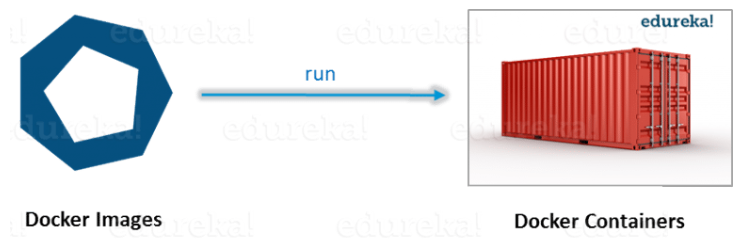
\includegraphics[height=3.5cm]{fig2-6}
	\caption{رابطه‌ی بین داکر ایمیج و داکر کانتینر}
	\label{تصویر 2-6}
\end{figure}


\subsubsection*{داکر رجستری}

داکر رجستری\LTRfootnote{Docker Registry} یک انبار ذخیره‌سازی اطلاعات و یک سیستم توزیع‌شده برای داکر ایمیج‌های نام‌گذاری شده می‌باشد. ایمیج‌ها با ورژن‌های مختلف به وسیله 
\lr{tag}
از یکدیگر تفکیک می‌شوند. داکر رجستری این قابلیت را دارد که ورژن‌های مختلف ایمیج را
\lr{pull}
کنید و بعد از اعمال تغییرات مناسب آن را 
\lr{push}
کنید. به عنوان نمونه 
\lr{Docker hub}
یک نمونه داکر رجستری است که این اجازه را به کاربران می‌دهد تا ایمیج‌های خود را در فضای ابری مهیا شده، بارگذاری و استفاده کنند.
\newline
\newline
با توجه به تعاریف ذکر شده معماری داکر را می‌توان به شکل 
\ref{تصویر 2-7}
تعریف کرد:
\begin{figure}[!h]
	\centering
	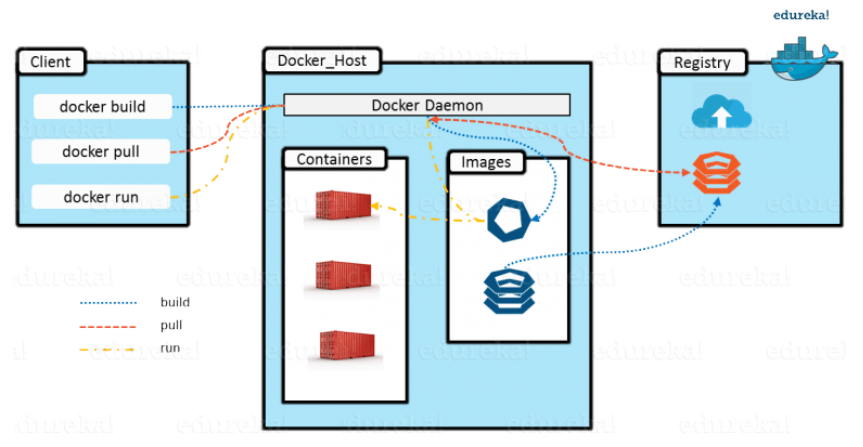
\includegraphics[height=8cm]{fig2-7}
	\caption{معماری داکر}
	\label{تصویر 2-7}
\end{figure}


\subsection{کوبرنتیز}

\subsubsection{مفاهیم اولیه}

کوبرنتیز یک هماهنگ‌کننده کانتینری متن باز، قابل حمل و قابل توسعه می‌باشد که برای اجرا و مدیریت کانتینرها و همچنین جهت تسهیل تنظیمات توسعه داده شده‌است. کوبرنتیز بر مبنای 15 سال تجربه گوگل در ساختن کانتینرها بنا شده‌است.
سؤال مهم این است که چه نیازی به استفاده از کوبرنتیز داریم؟ برای پاسخ به این سؤال بهتر است نگاهی به گذشته داشته باشیم و مسیر پیموده شده تا رسیدن به کوبرنتیز را دنبال کنیم.(شکل
\ref{تصویر 2-8}
)

%\cite{Kubernetes_What}

\begin{figure}[!h]
	\centering
	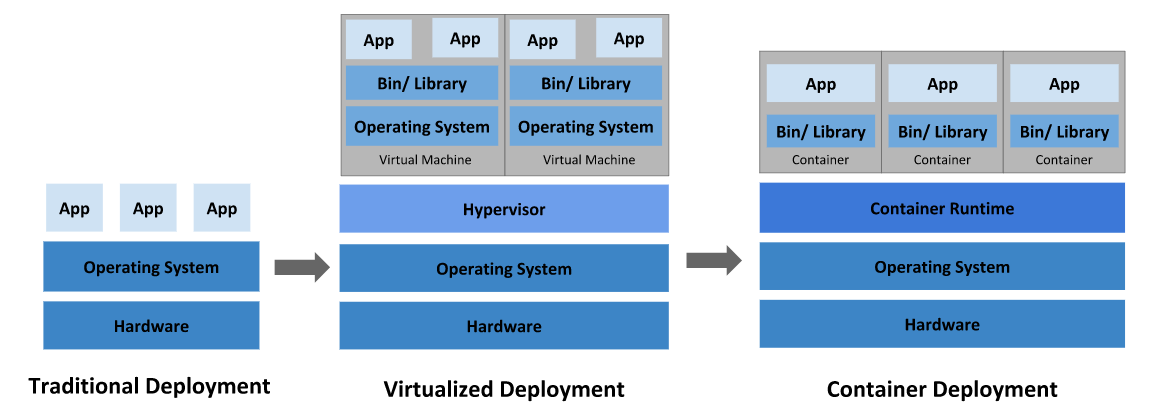
\includegraphics[height=5.5cm]{fig2-8}
	\caption{به سوی کوبرنتیز}
	\label{تصویر 2-8}
\end{figure}

\textbf{عصر استقرار سنتی}\LTRfootnote{Traditional deployment era}
: در آن دوره شرکت‌ها برنامه‌های کاربردی خود را بر روی سرورهای فیزیکی اجرا می‌کردند. در این حالت راه‌حلی برای تعیین حد‌و‌مرز برای استفاده از منابع توسط برنامه‌های کاربردی نبودو به همین دلیل مشکلات اختصاص منبع به وجود می‌آمد. به عنوان مثال اگر چند برنامه کاربردی بر روی سرور اجرا می‌شد ممکن بود یکی از برنامه‌ها بیشتر منابع را استفاده کند، درنتیجه برنامه‌های دیگر منبعی برای استفاده نداشتند. راه‌حل این مشکل اجرای یک برنامه کاربردی بر روی یک سرور فیزیکی بود. اما این روش باعث هدر‌دادن منابع زیادی می‌شود. همچنین قابلیت توسعه‌پذیری را سلب می‌کند. از طرفی نگه‌داری سرورهای فیزیکی برای شرکت‌ها بسیار دشوار است.  

\textbf{عصر استقرار مجازی}\LTRfootnote{Virtualized deployment era}
: به عنوان یک راه‌حل مجازی‌سازی معرفی شد. این راه‌حل اجازه می‌داد چندین ماشین مجازی را بر روی یک پردازده سرور فیزیکی اجرا کنیم. همچنین مجازی‌سازی اجازه ایزوله‌سازی بین برنامه‌های کاربردی را ایجاد می‌کرد و سطحی از امنیت اطلاعات را بین برنامه‌های کاربردی مختلف مهیا می‌کرد، به طوری که اجازه نمی‌داد یک برنامه کاربردی به اطلاعات برنامه کاربردی دیگر دسترسی داشته باشد. از فواید دیگر مجازی‌سازی می‌توان به استفاده بهتر از منابع موجود و مقیاس‌پذیری بهتر و همچنین کاهش هزینه‌های سخت‌افزار اشاره کرد. هر ماشین مجازی یک ماشین کامل است که همه اجزا لازم  را بر روی سخت‌افزار مجازی سازی‌ شده‌اش اجرا می‌کند.

\textbf{عصر استقرار کانتینری}\LTRfootnote{Container deployment era}
: کانتینرها شبیه ماشین‌های مجازی هستند با این تفاوت که آن خاصیت به اشتراک‌گذاری سیستم عامل را بین برنامه‌های کاربردی دارند. از این رو کانتینرها سبک وزن‌تر هستند. 
\newline

در نتیجه کانتینرها جهت اجرای برنامه‌های کاربردی بسیار مناسب هستند. در محیط تولید نیاز به مدیریت کانتینر در حال اجرا می‌باشد. همچنین نیاز داریم تا همواره از سلامتی کانتینر اطمینان حاصل کنیم. به عنوان نمونه اگر کانتینری از اجرا بایستد هر چه سریع‌تر کانتینر دیگر اجرا شود. چه بهتر است که این مدیریت توسط یک سیستم انجام گیرد. کوبرنتیز به همین دلیل به‌وجود‌آمده‌است. کوبرنتیز یک چارچوب را برای اجرای سیستم‌های توزیع‌شده و انعطاف‌پذیر اجرا می‌کند. همچنین نیازمندی‌های مقیاس پذیری، شکست کانتینر، الگوهای استقرار و بسیاری مسائل دیگر را مدیریت می‌کند. 
\newline
\newline
از ویژگی‌های کوبرنتیز می‌توان به موارد زیر اشاره کرد:
\begin{enumerate}
	\item 
	کشف سرویس و توزیع‌بار\LTRfootnote{Service discovery and load balancing}:\\
	کوبرنتیز بدون احتیاج به تغییر برنامه کاربردی این امکان را می‌دهد تا سرویس خود را ثبت نام کنید و اجازه دهید تا بقیه سرویس‌ها از وجود آن خبردار شوند. کوبرنتیز به هر کانتینر یک آدرس آی‌پی اختصاصی می‌دهد و برای هر گروه از کانتینرها یک نام دی‌ان‌اس اختصاص می‌دهد که امکان توزیع بار بین آن‌ها را فراهم می‌کند.
	\item 
	هدایت‌کردن انبارهای ذخیره اطلاعات\LTRfootnote{Storage orchestration}:\\
	کوبرنتیز این اجازه را می‌دهد تا به صورت خودکار انبارهای ذخیره اطلاعات سیستم را مقداردهی کنید.
	\item 
	تطبیق خودکار\LTRfootnote{Automated rollouts and rollbacks}:\\
	بدین معنی که حالت مورد انتظار خود را به کوبرنتیز معرفی می‌کنید و کوبرنتیز حالت فعلی را به حالت مورد انتظار تبدیل می‌کند.
	
	\item
	بسته‌بندی خودکار\LTRfootnote{Automatic bin packing}:\\
	با توجه به نیازمندی و منابع مورد‌نیاز هر کانتینر، کوبرنتیز به صورت اتوماتیک کانتینرها را بر روی گره‌ها قرار می‌دهد.
	\item
	ترمیم خودکار\LTRfootnote{Self-healing}:\\
	کوبرنتیز به صورت خودکار تمامی کانتینرهایی که موفق به اجرا نشوند را بازنشانی می‌کند. همچنین در صورتی که گره‌ای که کانتینر بر روی آن در حال اجرا است، دچار مشکل شود، کوبرنتیز تمامی کانتینرهای در حال اجرا بر روی آن را مجدداً روی گره‌های باقی‌مانده قرار می‌دهد.
	\item
	توسعه‌پذیری افقی:\\
	کوبرنتیز این امکان را می‌دهد تا برنامه کاربردی خود را به صورت اتوماتیک کوچک یا بزرگ کنید. همچنین این امکان را می‌دهد تا این کار را بر عهده‌ی خود کوبرنتیز قرار دهید و این کار به صورت خودکار انجام گیرد.
	
	\item
	مدیریت 
	\lr{secret}
	ها و تنظیمات\LTRfootnote{Secret and configuration management}:\\
	کوبرنتیز امکان ذخیره و مدیریت اطلاعات حساس مانند رمز‌عبورها، 
	\lr{OAuth tokens}
	, 
	\lr{ssh keys}
	را می‌دهد. می‌توانید بدون بازسازی کانتینرها، 
	\lr{secrets}
	و تنظیمات، محصول کاربردی را پیاده‌سازی و یا به‌روز کنید. این کار بدون نمایش‌دادن 
	\lr{secret}
	در فایل‌های تنظیمات انجام می‌گیرد.
	
\end{enumerate}

\newpage

\subsubsection{معماری کوبرنتیز}
اولین مرحله جهت کار کردن با کوبرنتیز شناخت معماری و اجزای آن است.

یک نود کوچک‌ترین جز سخت‌افزارهای محاسباتی در کوبرنتیز است. نود نماینده یک ماشین در خوشه است. در بیشتر سیستم‌های تولید، به احتمال زیاد نود یک ماشین فیزیکی در مرکز داده (‌دیتاسنتر) و یا یک ماشین مجازی بر روی ارائه‌دهندگان ابر\LTRfootnote{cloud provider} می‌باشد. تعریف یک نود به عنوان یک ماشین، ‌این اجازه را می‌دهد که یک لایه از مفاهیم را استفاده  کنیم. بدین معنا که نیاز نیست نگران مشخصات یکتا ماشین باشیم بلکه هر ماشین را مجموعه‌ای منابع مانند 
\lr{cpu}
و
\lr{gpu}
درنظر می‌گیریم که می‌توانند استفاده شوند. بدین ترتیب هر ماشین می‌تواند جایگزین ماشینی دیگر در دنیای کوبرنتیز شود.

اگرچه کارکردن با تک‌نودها می‌تواند مفید باشد اما این روش کوبرنتیز نیست. به طور کلی در کوبرنتیز ما یک خوشه\LTRfootnote{cluster} را به جای حالت‌های تک‌نودها درنظر می‌گیریم(شکل
\ref{تصویر 2-9}
). در کوبرنتیز نودها منابع خود را به اشتراک می‌گذارند تا یک ماشین قدرتمند‌تر شکل گیرد. وقتی برنامه‌های خود را بر روی خوشه مستقر می‌کنید، کارهای اجرایی برنامه به صورت هوشمندانه بر روی تک نودها توزیع می‌شود. اگر نودی اضافه یا حذف شود، خوشه کارها را بر روی نودها  جابه‌جا می‌کند. لازم به ذکر است برنامه و برنامه‌نویس با نحوه اجرای برنامه و توزیع آن بر روی نودها درگیر نیستند.

\begin{figure}[!h]
	\centering
	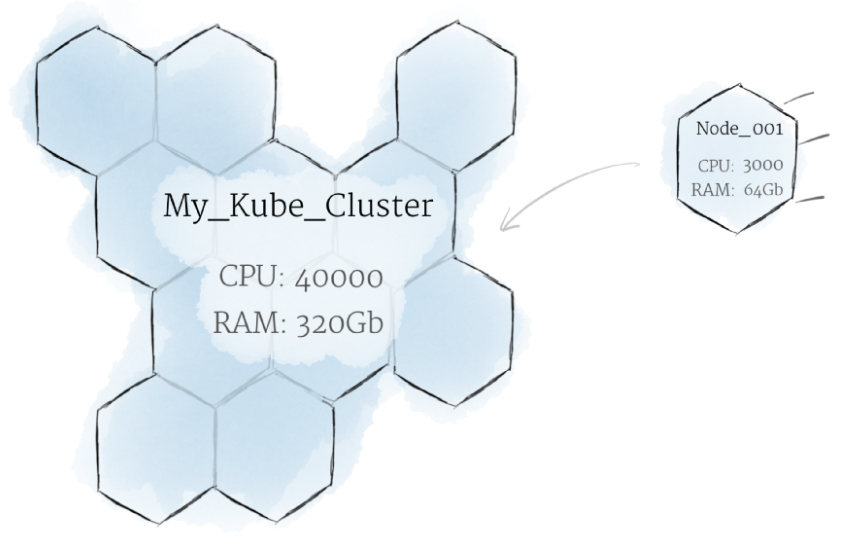
\includegraphics[height=7cm]{fig2-9}
	\caption{رابطه‌ی نود و خوشه در کوبرنتیز}
	\label{تصویر 2-9}
\end{figure}

تصویر (شکل 
\ref{تصویر 2-10}
)
معماری یک خوشه کوبرنتیز\LTRfootnote{Kubernetes Cluster}می‌باشد. از آن جایی که کوبرنتیز یک خوشه محاسباتی را پیاده می‌کند، همه چیز در داخل این خوشه کوبرنتیز اتفاق می‌افتد. این خوشه میزبانی یک نود با نام مستر\LTRfootnote{master} و نودهای دیگر با نام نود کارگر\LTRfootnote{worker node} را بر عهده دارد. همچنین خارج خوشه یک متعادل‌کننده بار\LTRfootnote{load balancer} وجود دارد که ترافیک خارجی را کنترل و بین نودها پخش می‌کند.  مستر کنترل خوشه و نودهای داخل آن را برعهده دارد. هر نود میزبان یک یا تعدادی پاد\LTRfootnote{pod} می‌باشد و هر پاد شامل گروهی از کانتیرها می‌باشد که برای یک هدف با یکدیگر در تعامل هستند.

\begin{figure}[!h]
	\centering
	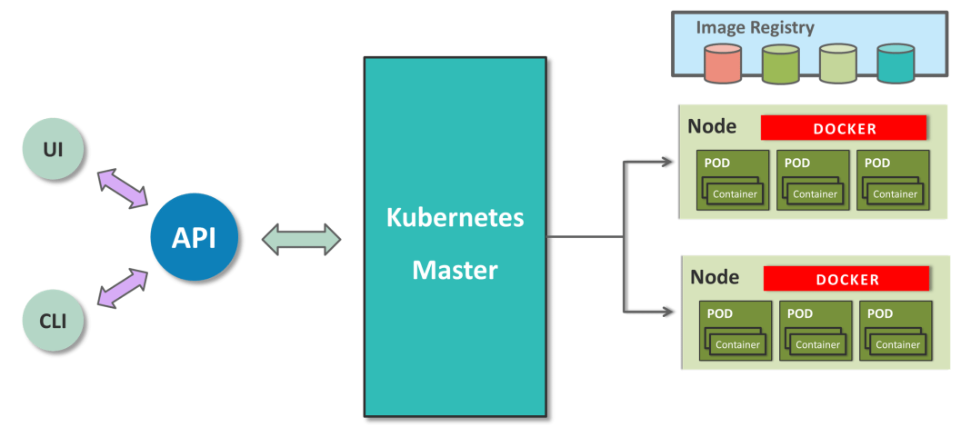
\includegraphics[height=5cm]{fig2-10}
	\caption{معماری خوشه کوبرنتیز}
	\label{تصویر 2-10}
\end{figure}

در نتیجه به طور کلی معماری خوشه‌ی کوبرنتیز (شکل
\ref{تصویر 2-11}
) دارای اجزا اصلی زیر می‌باشد:

\begin{enumerate}
	\item 
	نودهای مستر
	\item 
	نود‌های کارگر
	\item 
	مراکز ذخیره اطلاعات توزیع‌شده به صورت
	\lr{key-value}\LTRfootnote{ Distributed key-value store(etcd)}
\end{enumerate}

\begin{figure}[!h]
	\centering
	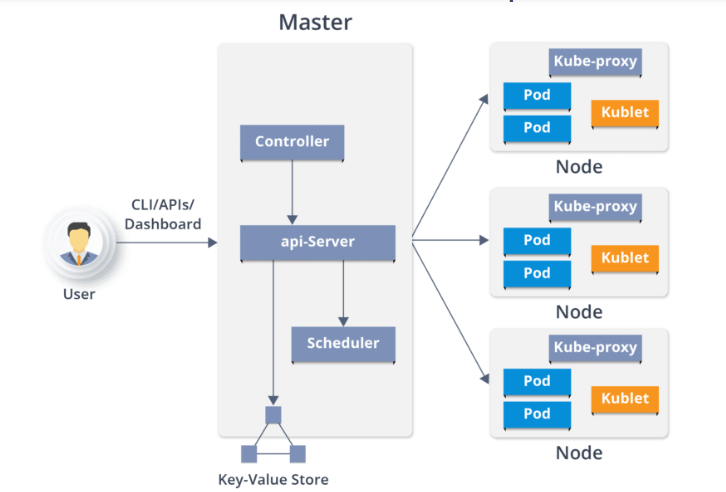
\includegraphics[height=7cm]{fig2-11}
	\caption{ معماری خوشه کوبرنتیز با جزییات هر بخش}
	\label{تصویر 2-11}
\end{figure}


\subsubsection*{گره مستر}
گره مستر را می‌توان یک نقطه شروع برای همه کارهای اجرایی که قرار است آن خوشه کوبرنتیز بر عهده داشته باشد، دانست. می‌توان برای چک کردن تحمل خطا بیش از یک نود مستر را در خوشه قرار داد. در این حالت نیز یکی از نودهای مستر به عنوان نود اصلی شناخته می‌شود و ما دستورات لازم را به آن اعمال می‌کنیم. تنها گره‌های مستر توانایی اجرای عملیات زمان‌بندی کانتینرها بر روی گره‌های کارگر یا خودشان را دارا می‌باشند. هر گره مستر یک رابط برنامه‌نویسی دارد که از طریق آن با رابط کنسولی و یا رابط تحت وب می‌توان با گره مستر ارتباط برقرار نمود.

در کوبرنتیز نودها به وسیله مستر ساخته و مدیریت می‌شوند. در واقع در مستر برنامه‌هایی اجرا می‌شوند، که این برنامه‌ها ساخت و اجرای نودها را کنترل می‌کنند. توسعه‌دهندگان برنامه‌های خود را در قالب فایل تنظیمات\LTRfootnote{config file} به مستر می‌دهند و مستر برنامه خواسته‌شده را در نودها پخش می‌کند.
\newline
\newline
گره مستر دارای چهار جز اصلی است که به تشریح آن‌ها می‌پردازیم:
\begin{enumerate}
	\item
	\lr{:Api server}\\
	تمام کارهای مدیریتی از طریق 
	\lr{api server}
	در گره مستر انجام می‌شود. تمام دستورات
	\lr{REST}
	که به
	\lr{api server}
	فرستاده می‌شوند در این قسمت اعتبارسنجی و پردازش می‌شوند. پس از اجرای درخواست، نتیجه به‌دست‌آمده در مراکز ذخیره اطلاعات توزیع‌شده ذخیره می‌شوند.
	\item
	زمان‌بند\LTRfootnote{scheduler}: \\
	این قسمت وظیفه زمان بندی کارها را برای گره‌های کارگر بر عهده دارد. همچنین اطلاعات مصرف منابع هر نود کارگر را در خود نگه می‌دارد.
	\item
	مدیر کنترل\LTRfootnote{controller manager}:\\
	یک
	\lr{daemon}\RTLfootnote{در سیستم عامل‌ها ، یک برنامه کامپیوتری است که  به جای آن که تحت کنترل مستقیم یک کاربر باشد، به عنوان یک پردازه در پس‌زمینه اجرا می‌شود.}
	است که وظیفه کنترل حلقه‌های بدون انتها را بر عهده دارد. همچنین وظیفه اجرای توابع چرخه زندگی\LTRfootnote{lifecycle} مانند ساخت
	\lr{namespace}
	و
	\lr{lifecycle}
	، جمع‌آوری زباله (باقی‌مانده) 
	\lr{event}
	ها، جمع‌آوری زباله (باقی‌مانده) پادهای خاتمه‌یافته، جمع‌آوری زباله (باقی‌مانده) پاک‌کردن‌های آبشاری، جمع‌آوری زباله (باقی‌مانده) نودها و ... را بر عهده دارد. از وظایف دیگر این قسمت تماشا‌کردن و دنبال‌کردن وضعیت مورد‌انتظار اشیا و وضعیت فعلی اشیا می‌باشد و زمانی که این دو وضعیت در شرایط برابر نباشند، حلقه اصلاحی را به سیستم اعمال می‌کند تا این دو وضعیت برابر شوند.
	\item
	\lr{:ETCD}\\
	یک مرکز ذخیره‌سازی توزیع‌شده به صورت
	\lr{key-value}
	می‌باشد که حالت خوشه را در خود نگه می‌دارد. هم می‌تواند قسمتی از نود مستر باشد و هم می‌تواند یک تنظیمات خارجی باشد. علاوه بر حالت خوشه جزییات تنظیمات خوشه را نیز در خود نگه‌داری می‌کند.
\end{enumerate}


\subsubsection*{گره کارگر}

یک سرور فیزیکی و یا یک ماشین مجازی می‌باشد که به وسیله پاد برنامه‌های کاربردی را اجرا می‌کند و به وسیله گره مستر کنترل می‌شود. 

\begin{figure}[!h]
	\centering
	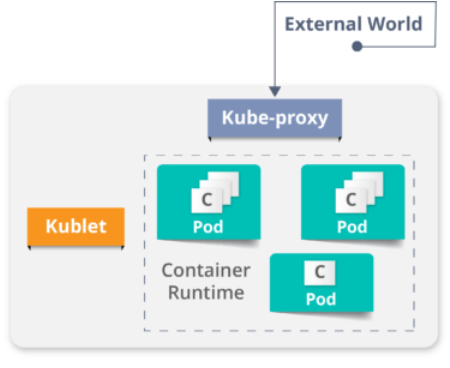
\includegraphics[height=7cm]{fig2-12}
	\caption{ معماری گره کارگر}
	\label{تصویر 2-12}
\end{figure}

گره کارگر دارای قسمت‌های زیر می‌باشد:(شکل
\ref{تصویر 2-12}
)
\begin{enumerate}
	\item
	\lr{:Container runtime}\\
	جهت اجرای چرخه زمان کانتینرها، گره کارگر به این قسمت نیازمند است. گاهی اوقات داکر به عنوان یک
	\lr{Container runtime}
	معرفی می‌شود اما در واقع داکر پلتفرمی می‌باشد که از کانتینرها به عنوان یک
	\lr{Container runtime}
	استفاده می‌کند. 
	
	\item
	\lr{:Kubelet}\\
	یک عامل است که با گره مستر ارتباط برقرار می‌کند و بر روی نودهای کارگر اجرا می‌شود. همچنین مشخصات فنی پادها را دریافت می‌کند و کانتینرهایی که به پادها مرتبط هستند را اجرا می‌کند. سپس از اجرا و سلامتی کانتیرها اطمینان حاصل می‌کند.
	\item
	\lr{:Kube-proxy}\\
	جهت ارتباط با شبکه (
	\lr{host sub-netting}
	) بر روی هر نود اجرا می‌شود و اطمینان حاصل می‌کند که سرویس‌ها برای قسمت‌های خارجی در دسترس هستند. همچنین به عنوان یک پروکسی شبکه و یک  متعادل کننده بار برای سرویس عمل می‌کند و مسیریابی شبکه را برای بسته‌های
	\lr{tcp}
	و
	\lr{udp}
	انجام می‌دهد. این پروکسی شبکه دائما به
	\lr{api server}
	گوش می‌دهد. برای هر سرویس یک مسیریابی انجام می‌دهد تا بتوان به آن دسترسی داشت.
	\item
	\lr{:Pod}\\
	شامل یک یا چند کانتینر است که کانتینرها از لحاظ منطقی با هم برابرند. پادها به عنوان یک واحد منطقی اجرا می‌شوند. پادها نیاز ندارند که بر روی یک ماشین مجازی اجرا شوند بلکه می‌توان هر کدام را بر روی یک ماشین مجازی متفاوت اجرا کرد. 
\end{enumerate}


\subsubsection{اشیا کوبرنتیز}

در فضای یک نود کارگر می‌توان از اشیا\LTRfootnote{object} مختلفی استفاده کرد. اشیا در کوبرنتیز موجودیت‌های ماندگار هستند. کوبرنتیز از این موجودیت‌ها برای نشان‌دادن حالت و وضعیت خوشه استفاده می‌کند. مهم‌ترین مواردی که این موجودیت‌ها توصیف می‌کنند شامل مشخص‌کردن برنامه‌های کاربردی کانتینرایز‌شده در حال اجرا، منابع در دسترس برای برنامه‌های در حال اجرا، سیاست‌هایی که مشخص می‌کند این برنامه‌ها چگونه رفتار کنند و ... می باشد. اشیا کوبرنتیز یک بار توسط توسعه‌دهنده ایجاد می‌شوند و سیستم کوبرنتیز دائما این اشیا را زیرنظر می‌گیرد و از وجود آن‌ها اطمینان حاصل می‌کند. به این خاصیت اصطلاحا 
\lr{record of intent}
می‌گویند. با ایجاد یک شی، به سیستم کوبرنتیز می‌گویید که می‌خواهید خوشه چگونه کار کند. بدین ترتیب حالت مورد انتظار خوشه را مشخص می‌کنید. جهت ساخت، اصلاح و یا حذف اشیا نیازمند 
\lr{kubernetes API}
هستید.

هر شی کوبرنتیز شامل دو قسمت تو‌در‌تو می‌باشد و هر قسمت خود یک شی است. این دو قسمت تنظیمات شی را اداره می‌کنند. این دو قسمت 
\lr{spec}
و
\lr{status}
نام دارند. قسمت 
\lr{spec}
که توسعه‌دهنده باید آن را مهیا کند، حالت مورد انتظار شی را توصیف می‌کند. قسمت 
\lr{status}
حالت حقیقی و فعلی شی را توصیف می‌کند که به وسیله سیستم کوبرنتیز تهیه و به‌روز می‌شود.

\begin{figure}[!h]
	\centering
	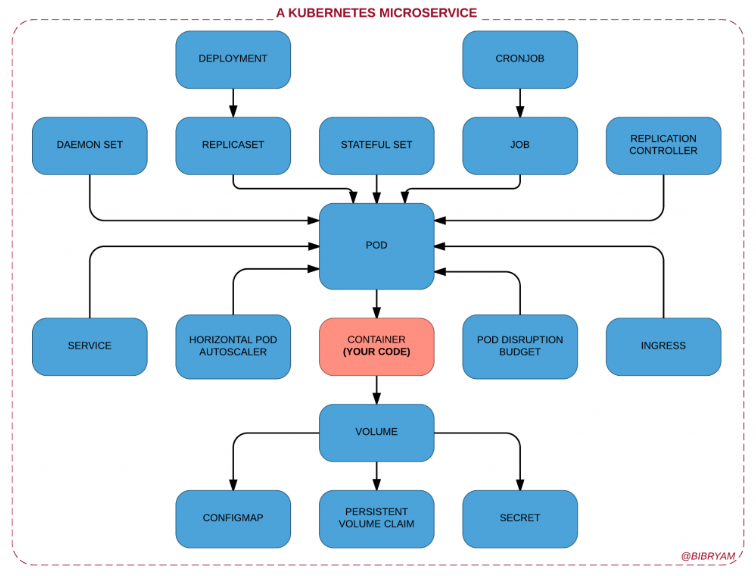
\includegraphics[height=10cm,width=\linewidth]{fig2-13}
	\caption{نمونه‌ای از اشیا موجود در کوبرنتیز}
	\label{تصویر 2-13}
\end{figure}

تعدادی از اشیا کوبرنتیز را معرفی می‌کنیم:
\cite{sanche_2018}
\begin{enumerate}
	\item
	\lr{:Pod}\\
	پاد گروهی از یک یا چند کانتینر با انبار ذخیره‌سازی \LTRfootnote{storage} و شبکه به‌اشتراک‌ گذاشته‌ شده می‌باشد. (شکل
	\ref{تصویر 2-14}
	) کوبرنتیز به طور مستقیم کانتینرها را اجرا نمی‌کند، بلکه یک یا چند کانتینر را  در ساختاری با نام پاد بسته‌بندی می‌کند. کانتینرهای داخل یک پاد دارای منابع یکسان به همراه شبکه محلی یکسان هستند. کانتینرها به آسانی با دیگر کانتینرهای داخل پاد ارتباط برقرار می‌کنند. این امر به این دلیل است که بر روی یک ماشین قرار دارند. البته همواره درجه‌ای از استقلال را نیز رعایت می‌کنند. پاد به عنوان واحدی برای تکثیر در کوبرنتیز شناخته می‌شود. اگر استفاده از برنامه کاربردی به اندازه‌ای شود که یک پاد توانایی تحمل بار آن را نداشته باشد، کوبرنتیز می‌تواند به گونه‌ای تنظیم شده باشد که در این حالت پاد موردنظر را تکثیر کند. حتی اگر برنامه‌ زیر بار سنگین نباشد، حالت استاندارد این است که چند کپی از پاد در یک لحظه در حال اجرا باشد تا تعادل بار و کنترل شکست آسان‌تر شود.
	پادها توانایی نگه‌داری چندین کانتینر را دارند اما ترجیح بر آن است که در هر پاد یک کانتینر نگه‌داری شود. چرا که پادها واحدی برای مقیاس‌پذیری هستند در نتیجه در صورت زیاد و یا کم‌ شدن تعداد پادها، همه کانتینرهای داخل پاد با هم زیاد و کم می‌شوند در‌حالی که ممکن است تنها لازم باشد مقیاس یکی از کانتینرها تغییر کند. در نتیجه این امر باعث هدر رفتن منابع و افزایش هزینه‌ها می‌شود. 
	
	\begin{figure}[!h]
		\centering
		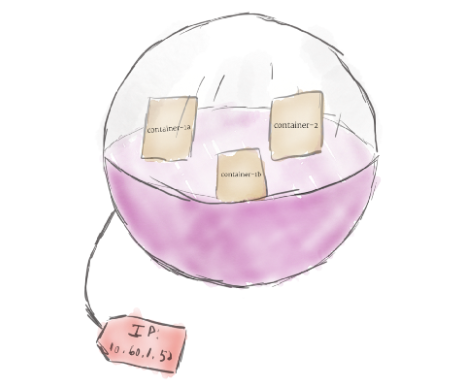
\includegraphics[height=6cm]{fig2-14}
		\caption{طرحی از یک پاد}
		\label{تصویر 2-14}
	\end{figure}
	
	\item
	\lr{:Replica set}\\
	یکی از مزایای کلیدی پادها این است که به توسعه‌دهندگان این اجازه را می‌دهند تا مجموعه‌ای از کانتینرها را به عنوان یک برنامه واحد گروه‌بندی و دسته‌بندی کنند و به آسانی با آن‌ها به عنوان یک حجم کار \LTRfootnote{workloads} کار کنند. پس از ساخت پادها، نمونه‌هایی از پادهای ساخته‌شده می‌توانند به صورت افقی مقیاس‌بندی\LTRfootnote{scale} شوند تا برنامه‌های چند کانتینری در دسترس باشند. برای مدیدیت مقیاس‌پذیری پادها، کوبرنتیز از یک 
	\lr{API object}
	استفاده می‌کند که 
	\lr{replica set}
	نام دارد.
	بر طبق مستندات کوبرنتیز، 
	\lr{replica set}
	ها این اطمینان را می‌دهند که تعداد مشخصی از کپی‌های پادها در هر زمان در حال اجرا باشند. 
	در 
	\lr{replica set}
	سه قسمت اصلی وجود دارد. (شکل
	\ref{تصویر 2-15}
	) قسمت اول 
	\lr{selector}
	نام دارد. وظیفه این قسمت انتخاب پاد موردنظر جهت مدیریت آن است. قسمت دوم 
	\lr{template}
	نام دارد. 
	\lr{replica set}
	با توجه به این قسمت پاد خواسته‌شده ساخته می‌شود. قسمت سوم 
	\lr{replicas}
	نام دارد که تعداد پادهای خواسته‌شده در این قسمت قرار می‌گیرد. با این که  
	\lr{replica set}
	ها توانایی مدیریت پادها را دارند اما قادر به به‌روز‌رسانی متحرک\LTRfootnote{rolling update} نیستند. به همین دلیل از تعریف جدیدی به نام 
	\lr{deployment}
	استفاده می‌شود. 
	\cite{nirmata_ReplicaSetsAndDeployments}
	
	\begin{figure}[!h]
		\centering
		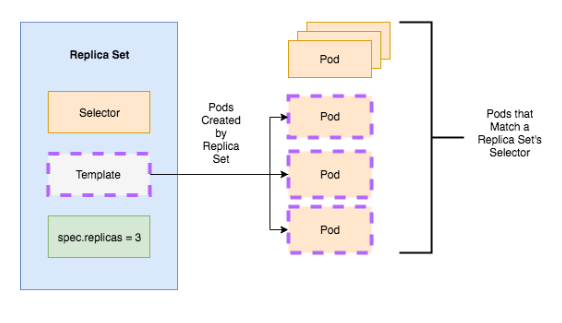
\includegraphics[height=7cm]{fig2-15}
		\caption{نحوه کارکرد 
			\lr{replica set}
		}
		\label{تصویر 2-15}
	\end{figure}
	
	\item
	\lr{:Deployment}\\
	با اینکه پادها اساسی‌ترین واحد محاسباتی در کوبرنتیز می‌باشند، اما به صورت مستقیم بر روی خوشه کوبرنتیز راه‌اندازی نمی‌شوند. در عوض پاد‌ها به وسیله‌ی یک لایه انتزاعی به نام 
	\lr{deployment}
	مدیریت می‌شوند. هدف اولیه 
	\lr{deployment}
	ها این است که مشخص کنند چند کپی از پاد در یک زمان باید در حال اجرا باشند.(شکل
	\ref{تصویر 2-16}
	) وقتی یک 
	\lr{deployment}
	به خوشه اضافه می‌شود، به صورت اتوماتیک ابتدا تعداد پادهای درخواست‌شده را راه‌اندازی می‌کند سپس بر آن‌ها نظارت می‌کند. اگر یک پاد بمیرد، 
	\lr{deployment}
	به صورت اتوماتیک دوباره آن را می‌سازد.
	
	\begin{figure}[!h]
		\centering
		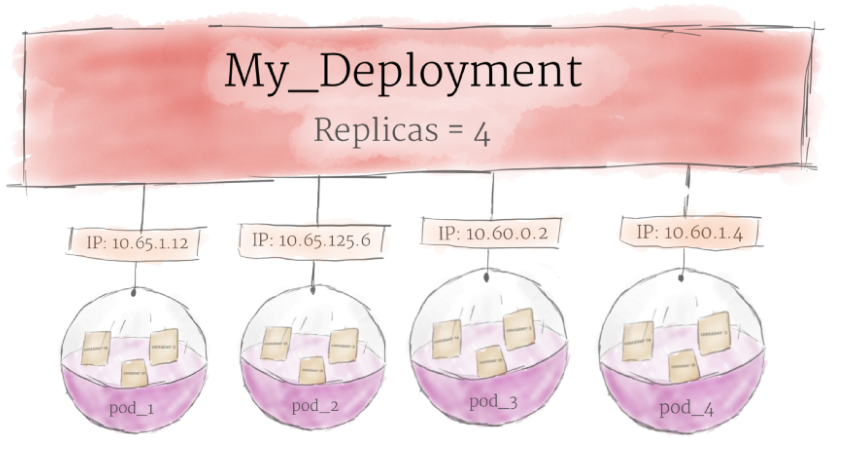
\includegraphics[height=5cm]{fig2-16}
		\caption{طرحی از یک 
			\lr{deployment}
		}
		\label{تصویر 2-16}
	\end{figure}
	
	از نگاهی دیگر 
	\lr{deployment}
	، پادها و 
	\lr{replica set}
	ها را بسته‌بندی می‌کند و روشی اعلامی
	\LTRfootnote{declarative method}
	برای به‌روز‌رسانی حالات آن‌ها مهیا می‌کند. (شکل
	\ref{تصویر 2-17}
	)
	
	\begin{figure}[!h]
		\centering
		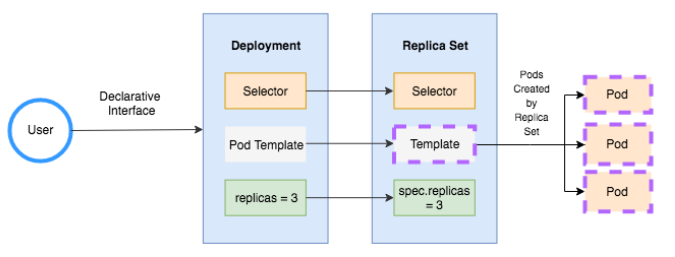
\includegraphics[height=5.5cm]{fig2-17}
		\caption{روش اعلامی ایجاد شده توسط 
			\lr{deployment}
		}
		\label{تصویر 2-17}
	\end{figure}
	
	
	\item
	\lr{:Service}\\
	یک مفهوم است که مجموعه‌ی منطقی از پادها و سیاست‌های دسترسی به آن‌ها را تعریف می‌کند. 
	\lr{Service}
	ها یک نقطه پایان\LTRfootnote{endpoint} برای پادها مشخص می‌کنند تا بتوانیم به آن‌ها دسترسی داشته باشیم و بدانیم در چه وضعیتی هستند. 
	
	\item
	\lr{:Storage class}\\
	راهی برای توصیف کلاس‌های انبار ذخیره توسط مدیران تهیه می‌کند. 
	\item
	\lr{:Persistent Volumes}\\
	اگر یک برنامه اطلاعات خود را در یک فایل محلی در نود ذخیره کند، زمانی که  برنامه به هر دلیلی به نود دیگر انتقال پیدا می‌کند، تضمینی وجود ندارد که اطلاعات در دسترس باشند. به همین علت می‌توان گفت انبارهای ذخیره‌سازی که در نودها وجود دارند به عنوان حافظه‌های موقت عمل می‌کنند و داده‌هایی در آن‌ها جا می‌گیرند پایدار نیستند. برای ذخیره اطلاعات به صورت دائمی کوبرنتیز از 
	\lr{Persistent Volumes}
	استفاده می‌کند. در نتیجه جهت مدیریت مصرف منابع، 
	\lr{Persistent Volume}
	ها را به خوشه‌ها اضافه می‌کنیم. 
	\lr{Persistent Volume}
	ها چرخه حیاتی دارند و مستقل از پادهایی هستند که به آن‌ها متصل می‌شوند.(شکل
	\ref{تصویر 2-18}
	)
	
	\begin{figure}[!h]
		\centering
		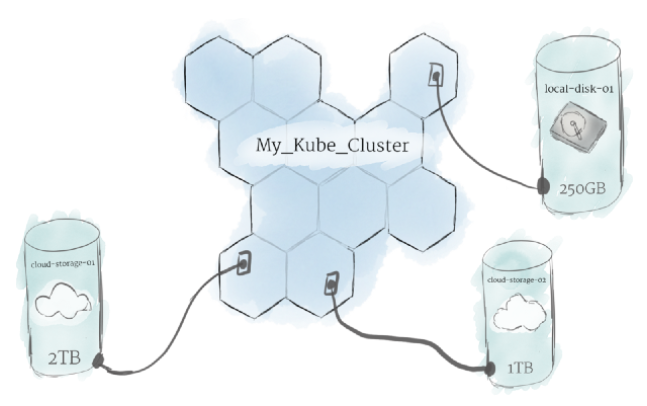
\includegraphics[height=6.5cm]{fig2-18}
		\caption{طرحی از  
			\lr{Persistent Volume}
		}
		\label{تصویر 2-18}
	\end{figure}
	
	
	\item
	\lr{:Persistent Volume Claim}\\
	یک تعریف انتزاعی از 
	\lr{Persistent Volume}
	می‌باشد. 
	\lr{Persistent Volume}
	ها منابع فیزیکی زیرساخت‌ها می‌باشند. کوبرنتیز جهت پنهان‌کردن جزییات از توسعه‌دهندگان این مفهوم را استفاده می‌کند. با استفاده از این مفهوم می‌توان تعاریف فیزیکی تعریف‌شده توسط 
	\lr{Persistent Volume}
	و
	\lr{Storage class}
	را پنهان کرد.
	
	\item
	\lr{:Ingress}\\
	به صورت پیش فرض کوبرنتیز پادها را از محیط بیرون مستقل و ایزوله کرده است. اگر می خواهید کانالی برای ارتباط پادها با فضای بیرون ایجاد کنید از
	\lr{Ingress}
	باید استفاده کنید.(شکل
	\ref{تصویر 2-19}
	)
	\begin{figure}[!h]
		\centering
		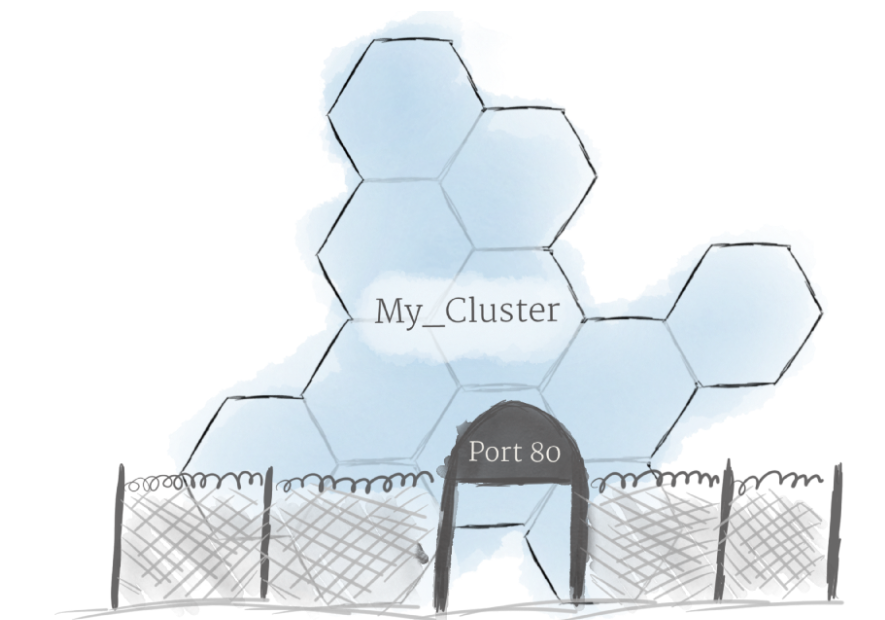
\includegraphics[height=6.5cm]{fig2-19}
		\caption{طرحی از  
			\lr{Ingress}
		}
		\label{تصویر 2-19}
	\end{figure}
	
\end{enumerate}


\subsubsection{ابزارهای کوبرنتیز}

در مدت کوتاه تقریبا دو ساله، کوبرنتیز از رقبایش به عنوان یک هدایت‌کننده کانتیری پیشی گرفته و به سرعت به عنوان مشهورترین ارائه‌دهنده راه‌حل‌های کانتینری
\LTRfootnote{container solution provider}
شناخته شده‌است. در این میان ابزارهایی به عنوان متمم سیستم کوبرنتیز به‌وجود آمده‌اند. به بررسی تعدادی از آن‌ها می‌پردازیم:
\begin{enumerate} 
	
	\item
	\lr{:Kubectl}\\
	یک ابزار خط فرمان
	\LTRfootnote{command line}
	جهت کنترل مدیریت خوشه‌ها می‌باشد.	
	
	\item
	\lr{:Kubeadm }\\
	یک ابزار خط فرمان و تامین‌کننده امنیت خوشه کوبرنتیز زمانی که در ماشین فیزیکی و یا مجازی و یا سرویس ابری در حال اجرا است. 	
	\item
	\lr{:Kubefed}\\
	یک ابزار خط فرمان جهت اداره کردن خوشه‌های به‌هم پیوسته (ترکیب شده) 	
	\item
	\lr{:Minikube}\\
	ابزاری جهت اجرای یک خوشه تک نود به صورت محلی با هدف توسعه و تست محصول. همچنین این ابزار دارای یک داشبورد تحت وب است که اطلاعات خوشه ساخته شده را به صورت بصری در اختیار قرار می‌دهد.
	
	\item
	\lr{:Helm}\\
	ابزار مدیریت پکیج‌هایی است که برای کوبرنتیز تنظیم شده‌اند. این منابع از پیش تنظیم شده با نام مستعار
	\lr{kubernetes charts}
	شناخته می‌شوند. می‌توان به کمک
	\lr{helm}
	پکیچ‌ها و منابعی که به صورت شخصی می‌سازیم را به اشتراک بگذاریم. همچنین می‌توانیم محصولات‌مان را به‌روز کنیم. 	
	
	\item
	\lr{:Kompose}\\
	ابزاری است که به کاربران کمک می‌کند فایل
	\lr{docker compose}
	خود را به شکل اشیا کوبرنتیز تبدیل کنند.    	
	
	
\end{enumerate}

ابزارهای ذکر‌شده بخش کوچکی از ابزارهای ساخته شده برای کوبرنتیز هستند. در زمینه‌های مختلفی مانند مانیتوریگ، تست کردن، دسترسی به منابع، امنیت، توسعه و ... می‌توان ابزارهای متعددی یافت که توسط شرکت‌های متعدد در حال توسعه هستند.

یکی از ابزارهای بسیار مهم در دنیای کوبرنتیز، ابزار
\lr{Prometheus}
می‌باشد که یک سیستم متن باز جهت نظارت\LTRfootnote{monitoring} و هشدار\LTRfootnote{alerting} است. از جمله مشخصات اصلی این ابزار می‌توان به موارد زیر اشاره کرد:
\cite{prometheus_overview}

\begin{enumerate}
	\item
	مدل داده‌ی چند بعدی به همراه داده‌های در طول زمان که به صورت
	\lr{key/value}
	هستند
	\item
	دارای
	\lr{PromQL}
	، یک زبان پرس‌‌و‌جو \LTRfootnote{query} منعطف جهت نفوذ به ابعاد داده
	\item
	دارای گره‌های سرور خودمختار ( انبارهای ذخیره‌سازی توزیع‌شده نمی‌باشند )
	\item
	اطلاعات بر حسب سری زمانی نگه‌داری می‌شوند
	\item
	چندین مدل جهت نشان دادن اطلاعات موجود است. 
\end{enumerate}


\subsubsection{کوبرنتیز در محیط توسعه و محیط محصول}
تفاوت‌های بسیاری در استفاده از کوبرنتیز در محیط توسعه \LTRfootnote{development} و در محیط محصول\LTRfootnote{production} می‌باشد. در محیط توسعه ابزاری به نام
\lr{minikube}
وجود دارد که تنها هدف آن نصب یک خوشه بر روی کامپیوتر محلی می‌باشد. در حالی که برای برپا کردن یک محصول کوبرنتیز در محیط محصول نیاز به
\lr{managed solution}
ها داریم.
\lr{managed solution}
ها منابع خارجی ارائه‌کننده ابر\LTRfootnote{cloud provider} مانند
\lr{google cloud}
و
\lr{amazon AWOS}
می‌باشند که خوشه کوبرنتیز را نصب می‌کنند و به صورت امن خوشه را در حالت اجرا نگه می‌دارند. البته این امر بدین معنا نیست که بدون
\lr{managed solution}
ها اجرای محصول کوبرنتیز در محیط محصول ناممکن باشد. بلکه بدون این ابزارها توسعه محصول کار دشوارتری می‌باشد و نیازمند تنظیمات پیچیده‌تری است.

\section{مدل‌های رایانش ابری}

رایانش ابری یک الگو است که در آن خدمات رایانشی مانند حافظه ذخیره سازی، سرورهای رایانشی و پایگاه داده ها از طریق اینترنت توسط ارائه‌دهندگان ابری\LTRfootnote{cloud providers} به کاربران ارائه می‌شود. ارائه دهندگان برای استفاده از خدمات، هزینه را به ازای هر بار استفاده، محاسبه می‌کنند. این مدل صورتحساب شبیه به خدمات روزانه مانند برق، گاز و آب است. محیط رایانش ابری از یک ارائه دهنده ابر تشکیل شده است که منابع بر اساس تقاضا و بسیار مقیاس پذیر را از طریق اینترنت برای مشتریان فراهم می‌کند. این منابع می‌توانند یک برنامه، یک پایگاه داده یا یک ماشین مجازی ساده و بدون سیستم عامل باشند. ارائه دهنده مسئولیت بیشتر مدیریت زیرساخت ها را بر عهده دارد. با این حال، کاربر هنوز وظیفه معدود کارهایی مانند انتخاب سیستم عامل، ظرفیت و اجرای برنامه را بر عهده دارد. ارائه دهنده می‌تواند ضمن دستیابی به چند اجازه، سریعاً منابع را مستقر و مقیاس کند. در حالی که، هزینه و زحمت های مدیریتی سمت کاربر به شدت کاهش می‌یابد.

تحولات رایانش ابری را می‌توان به مدل‌های زیر تقسیم کرد:

\begin{itemize}
	
	\item \textbf{زیرساخت به عنوان سرویس\LTRfootnote{Infrastructure as a Service} (\lr{IaaS})} یک مدل رایانش ابری است، که در آن ارائه دهندگان، زیرساخت را مانند سرورها، پایگاه داده و فضای مرکز داده ها ارائه می‌دهند. با استفاده از این مدل، کاربر نیازی به نگرانی در مورد راه اندازی، تعمیر، نگهداری و مقیاس پذیری زیرساخت‌ها ندارد.
	
	\item \textbf{بستر نرم‌افزاری به عنوان سرویس\LTRfootnote{Platform as a Service} (\lr{PaaS})} متشکل از ارائه دهنده خدماتی است که بستر رایانشی آماده به همراه راه حل های کاربردی را به کاربر ارائه می‌دهد و باعث صرفه جویی در زمان راه اندازی می‌شود. مشتری می‌تواند با تعامل کمتر با واسطه برنامه های کاربردی را توسعه دهد و به سرعت پیاده‌سازی کند. مشتری همچنین نیازی به نگرانی در مورد نرم افزار، پیکربندی شبکه (\lr{provisioning}) و میزبانی (\lr{hosting}) ندارد.
	
	\item \textbf{نرم‌افزار به عنوان سرویس\LTRfootnote{Software as a Service} (\lr{SaaS})} یک مدل رایانش ابری است که در آن کاربران بدون هیچ گونه نگرانی در مورد پیاده‌سازی و مدیریت از برنامه های مبتنی بر وب مستقر در سرورهای ابری بهره مند می‌شوند. با استفاده از یک مرورگر وب به این برنامه های میزبان ابری دسترسی پیدا می‌کنند. در این مدل کاربران از خدماتی با شروع سریع، تقاضا محور، موقعیت مکانی مستقل و مقیاس پذیری پویا بهره‌مند می‌شوند. با این حال، این رویکرد این مشکل را دارد که کاربر کنترل بسیار کمتری روی آن دارد.
	
	\item \textbf{رایانش بدون سرور} آخرین مدل رایانش ابری است که به طور خاص برای برنامه های گذرا (\lr{ephemeral})، فاقد وضعیت (\lr{stateless}) و رویداد محور(\lr{event based}) ساخته شده است. مدل رایانش بدون سرور مبتنی بر مقیاس پذیری افقی براساس تقاضا است زیرا برنامه های میزبانی شده نیاز به مقیاس شدن با سرعت بالا دارند. این مدل همچنین از رویکرد "\lr{pay as you go}" رایانش ابری استفاده می‌کند و صورتحساب کاربران بر اساس استفاده با دقت میلی‌ثانیه حساب می‌شود. تعریف رسمی‌تر از رایانش بدون سرور این است: "معماری های بدون سرور به برنامه هایی اطلاق می‌شوند که بستگی به خدمات شخص ثالث بستگی دارد (\lr{Backend} به عنوان سرویس یا \lr{BaaS}) یا به کدی که در کانتینرهای گذرا اجرا می‌شود (تابع به عنوان سرویس یا \lr{FaaS}).
	
\end{itemize}

در شکل مدل‌های رایانش ابری نشان داده شده و همچنین بخش‌های مدیریت شده توسط ارائه دهنده مشخص شده‌ است.

\begin{figure}[!h]
	\centering
	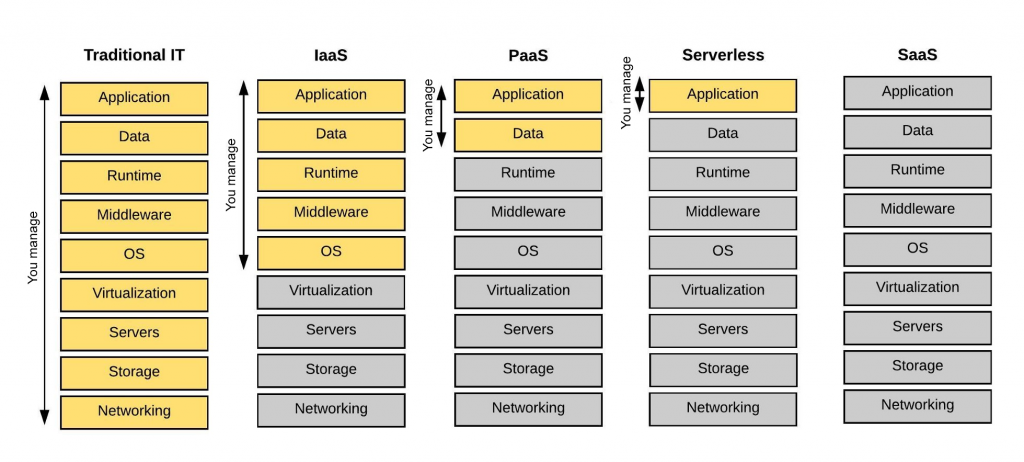
\includegraphics[height=7cm]{Images/cloud-computing-service-models}
	\caption{مدل‌های رایانش ابری}
	\label{تصویر 2-1}
\end{figure}

\section{رایانش بدون سرور}

تعریف اصطلاح بدون سرور دشوار است، زیرا این اصطلاح گمراه کننده است و تعریف آن هم بر مفاهیم دیگر مانند بستر نرم افزاری به عنوان سرویس (\lr{PaaS}) و نرم افزار به عنوان سرویس (\lr{SaaS}) همپوشانی دارد. بدون سرور بین این دو مفهوم قرار دارد، جایی که توسعه دهنده کنترل برخی زیرساخت های ابر را از دست می‌دهد، اما همانطور که در شکل  توضیح داده شده است، بر روی کد برنامه کنترل دارد. مفاهیم بدون سرور به دو دسته تقسیم می‌شوند:

\subsection{\lr{Backend} به عنوان سرویس (\lr{BaaS})}

در مدل \lr{BaaS}\LTRfootnote{Backend as a Service} منطق سمت سرور دیگر توسط کاربر پیاده‌سازی و مدیریت نشده و در عوض از سرویس های ارائه دهنده استفاده می‌شود. این مدل بسیار نزدیک به مفهوم نرم افزار به عنوان سرویس (\lr{SaaS}) است تا سر و کار داشتن با ماشین های مجازی و کانتینرها. در این مدل، برنامه ها به اجزای کوچک تر تقسیم می‌شوند و تعدادی از این اجزاء کاملا با محصولات برون‌سپاری شده پیاده‌سازی می‌شوند.

سرویس های \lr{BaaS} دارای دامنه های عمومی‌هستند و از راه دور و از طریق \lr{API}\LTRfootnote{Application Programming Interface} مورد استفاده قرار می‌گیرند. این سرویس ها بیشتر مورد توجه توسعه دهندگان برنامه تلفن همراه و صفحات وب ثابت قرار گرفته است زیرا به راحتی می‌توانند برای انجام کارهای مورد نیازشان از این سرویس ها استفاده کنند. برای مثال \lr{Firebase} گوگل یک پایگاه داده است که کاملا توسط خود گوگل مدیریت می‌شود و از آن مستقیماً می‌توان در هر برنامه کاربردی و بدون نیاز به هیچ سروری استفاده کرد.

نمونه دیگر سرویس های \lr{BaaS} استفاده از منطق برنامه ای است که توسط تیم های دیگر پیاده‌سازی شده. به عنوان مثال سرویس هایی مانند \lr{Auth0} و \lr{Cognito} برای احراز هویت کاربران و مدیریت آن ها وجود دارند که برنامه های وب و تلفن همراه می‌توانند از آن استفاده کنند بدون این که نیاز داشته باشند تیم توسعه آن ها حتی قسمتی از این منطق را خودشان پیاده‌سازی کنند.

\lr{BaaS} به خاطر رشد در زمینه  توسعه برنامه های کاربردی تلفن همراه معروف شد و گاهی اوقات به \lr{MBaaS}\LTRfootnote{Mobile Backend as a Service} یا \lr{Backend} تلفن همراه به عنوان سرویس شناخته می‌شد. اما این مفهوم به \lr{backend} برای برنامه های کاربردی تحت وب و موبایل محدود نمی‌شود و به عنوان مثال می‌توان از سرویس هایی برای مدیریت سیستم فایل و ذخیره سازی داده و حتی آنالیز گفتار استفاده کرد که کاملا توسط شرکت دیگری ارائه و مدیریت می‌شوند. همچنین از این سرویس‌ها در سمت سرور نیز می‌توان بهره برد.

\subsection{تابع به عنوان سرویس (\lr{FaaS})}

در مدل سرویس دهی \lr{FaaS}\LTRfootnote{Function as a Service}، منطق سمت سرور همچنان توسط خود برنامه نویسان نوشته شده و کنترل می‌شود. اما برنامه ها در کانتینرهای فاقد وضعیت و گذرایی اجرا می‌شوند و که به وسیله رویدادها ایجاد شده اند.

این مفهوم در بسیاری از موارد برای تعریف کردن مفهوم بدون سرور استفاده می‌شود و بسیاری از افراد آن دو را به اشتباه به جای یکدیگر به کار می‌برند. اگرچه \lr{FaaS} به نسبت بقیه مفاهیم بدون سرور جدیدتر است و برای پیاده‌سازی پروژه تمرکز ما بر روی این مدل سرویس بیشتر خواهد بود، بنابراین بیشتر به توضیح کارکرد آن خواهیم پرداخت.
هنگامی‌که ما می‌خواستیم برنامه سمت سرور را به روش های متداول قدیمی‌پیاده‌سازی کنیم، ابتدا با یک سرور میزبان، یک ماشین مجازی یا حتی یک کانتینر شروع به کار می‌کردیم. سپس برنامه خود را درون آن میزبان مستقر می‌کردیم. چنانچه میزبان یک ماشین مجازی یا کانتینر بود، برنامه ما به عنوان یک پردازه سیستم عامل اجرا می‌شد. معمولا برنامه ما متشکل بود از کدهایی که برای انجام عملیات های مختلف و مرتبط با هم نوشته شده بودند.

\lr{FaaS} این نوع پیاده‌سازی را تغییر داد. به این صورت که میزبان و پردازه ی برنامه از این مدل حذف شدند و تمرکز بر پیاده‌سازی منطق برنامه به صورت عملیات ها و تابع های جداگانه قرار گرفت. این تابع ها پس از توسعه به صورت جداگانه بر روی بستر ‌\lr{FaaS} قرار گرفته و اجرا می‌شوند. این تابع ها اما مانند یک پردازه سرور نیستند که  پیوسته فعال باشند و همیشه در وضعیت \lr{idle} قرار داشته باشند تا اینکه زمان اجرای آن ها برسد و به صورت قدیمی‌اجرا شوند. در عوض بستر بدون \lr{FaaS} طوری ساخته شده که برای هر تابع منتظر رویداد مربوط به آن بماند. زمانی که آن رویداد رخ داد، بستر از تابع مربوط به آن یک نمونه می‌سازد، سپس آن نمونه را با پارامترهای رویداد اجرا می‌کند. هنگامی‌که اجرای تابع به اتمام رسید، بستر \lr{FaaS} آزاد است که آن را حذف کند، اما ممکن است آن را برای بهینه سازی مدتی نگه دارد تا اگر رویداد جدیدی رخ داد نخواهد آن را از ابتدا بسازد.

\lr{FaaS} یک رویکرد رویداد محور\LTRfootnote{event-driven} است که علاوه بر ارائه یک بستر برای میزبانی و اجرای توابع با بسیاری از منابع رویدادی همگام و ناهمگام ادغام شده است. برای مثال \lr{HTTP API Gateway} یک منبع رویداد همگام است و صف پیام، عملیات ذخیره سازی یا رویدادهای برنامه ریزی شده، از منابع رویداد ناهمگام هستند.

از نظر سطحی، \lr{BaaS} و \lr{FaaS} کاملاً متفاوت هستند. مورد اول برون‌سپاری کامل اجزای برنامه به صورت جداگانه است و مورد  دوم یک محیط میزبانی جدید برای اجرای کد شخصی افراد است. پس چرا آن ها با هم زیر مجموعه مفهوم بدون سرور قرار می‌گیرند؟

دلیل اصلی این است که در هر دو مورد توسعه دهنده نیاز نیست که مدیریت زیرساخت های سرور خودش و یا پردازه های سرور را در نظر بگیرد. بلکه تمامی منطق برنامه در یک محیط عملیاتی کاملا \lr{elastic} اجرا می‌شود و وضعیت برنامه نیز در محیطی متشابه ذخیره می‌گردد. با تغییر تقاضا روی سرور، بستر بدون سرور بر این اساس تعداد ظرفیت سرورها را افزایش داده و یا کاهش می‌دهد، بدون اینکه لازم باشد برنامه نویسی توسط توسعه دهنده انجام شود. هزینه میزبانی یک سرویس بدون سرور معمولاً متناسب با تعداد درخواست های اجرای تابع ها محاسبه می‌شود. به عبارت دیگر بدون سرور به این معنی نیست که واقعا سروری در کار نباشد بلکه بدین معنی است که دیگر نیازی نیست نگران سرور باشید!

چالش اصلی بستر بدون سرور ارائه همه این موارد است در حالی که باید با الزاماتی از قبیل هزینه، تحمل خطا و مقیاس پذیری کنترل شود. چالش هایی که یک بستر بدون سرور برای اینکه بتواند رقابتی باشد باید بر آن غلبه کند عبارتند از:

\begin{itemize}
	
	\item سرعت برای شروع اجرای یک تابع و پردازش رویداد.
	
	\item صف رویدادها و سازگاری متناسب با آن ها. با توجه به ورود رویداد ها و وضعیت فعلی صف، باید برنامه زمانبندی اجرای تابع تنظیم و مدیریت شود تا منابع را از توابعی که در حال اجرا نیستند پس بگیرد.
	
	\item چگونگی مقیاس پذیری و مدیریت خطاها را به دقت در نظر بگیرد.
	
\end{itemize}

همانطور که در شکل مشاهده می‌شود، از زمان شکل گیری مفهوم بدون سرور، محبوبیت آن بسیار افزایش یافته است و انتظار می‌رود که این رشد همراه با رشد \lr{IoT} (شکل 2.1) ادامه داشته باشد. رشد تخمین زده شده آینده بدون سرور در شکل 2.7 قابل مشاهده است.

\begin{figure}[!h]
	\centering
	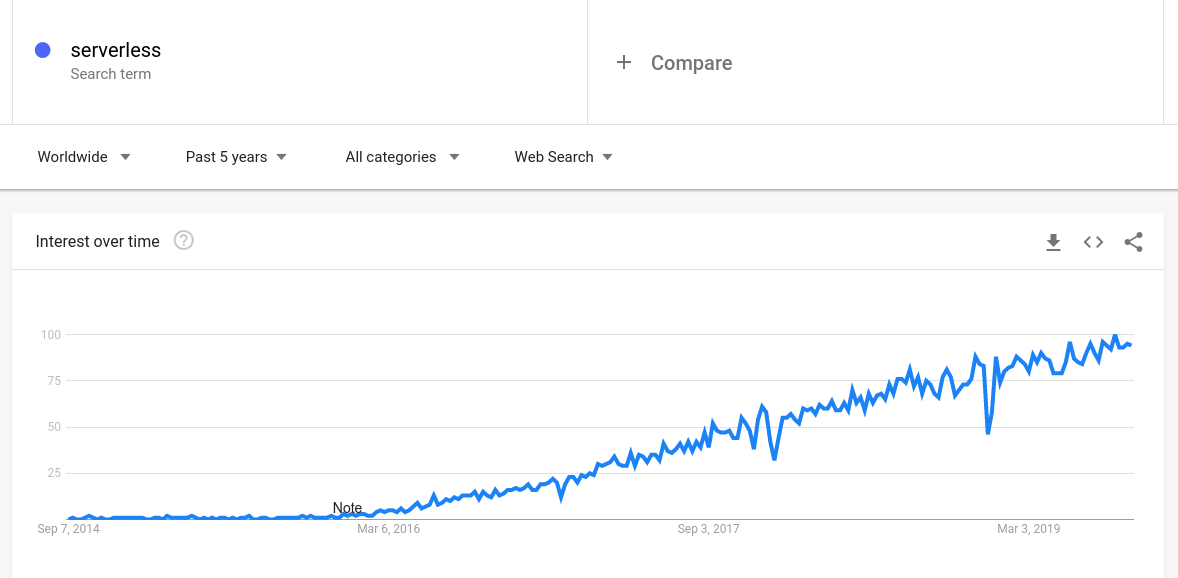
\includegraphics[height=8cm]{Images/serverless_google_trends}
	\caption{افزایش محبوبیت کلمه \lr{serverless} ‌‌در \lr{‌Google Trends} طی سه سال اخیر}
	\label{تصویر 2-1}
\end{figure}

\subsection{راه حل‌ها و بسترهای ابری موجود}

\begin{itemize}
	
	\item \textbf{\lr{Amazon lambda}}  اولین بستری که مدل سرویس بدون سرور را پیاده‌سازی کرد و معیارهای آن از جمله  قیمت گذاری، مدل برنامه نویسی، نحوه استقرار، محدودیت منابع، امنیت و مانیتورینگ را به بازار معرفی کرد. \lr{Lambda} از زبان های برنامه نویسی \lr{Node.js}، \lr{Python}، \lr{Java}  و \lr{C\#} پشتیبانی می‌کند. با توجه به این که این بستر در این زمینه پیشگام بوده است به عنوان اولین و بهترین راه حل انتخاب می‌شود و تعداد زیادی از شرکت های بزرگ از سرویس های این بستر استفاده می‌کنند.
	
	\item \textbf{\lr{Google Cloud Functions}}   در حال حاضر این بستر بسیار محدود است و تنها از زبان \lr{JavaScript} که در محیط استاندارد \lr{Node.js} نوشته شده باشد پشتیبانی می‌کند و تنها به رویدادهای سرویس \lr{Google Cloud} یا درخواست های \lr{HTTP} پاسخ می‌دهد. همچنین این بستر هنوز در فاز بتا است و نسخه نهایی آن منتشر نشده است.
	
	\item \textbf{\lr{Microsoft Azure Functions}}  بستر بدون سرور متن بازی را ارائه می‌دهد که کد آن در \lr{Github} موجود است. تابع های ارائه شده توسط توسعه دهنده با \lr{HTTP webhook} که با سرویس های بستر ادغام شده است اجرا می‌شوند. این بستر نیز از زبان های محدودی پشتیبانی می‌کند.
	
	\item \textbf{\lr{OpenLambda}}  بستر بدون سرور و متن باز جدیدی است که کد آن در \lr{Github} موجود است. این بستر در مواردی مشکل دارد که توسعه دهندگان آن در حال رفع آن هستند:
	راه اندازی بسیار آهسته \lr{runtime} های زبان‌های برنامه نویسی
	استقرار حجم زیادی از کد
	پشتیبانی از حفظ وضعیت که با تابع های فاقد وضعیت پیاده شده باشد
	استفاده از پایگاه داده‌ها
	
	\item \textbf{\lr{OpenFaaS}}
	
	\item \textbf{\lr{OpenWhisk}}  کلیدی ترین ویژگی این بستر این است که می‌توان با اتصال تابع ها با یکدیگر ترکیبی از تابع ها را ساخت و آن را به عنوان تابع جدید ارائه داد. این بستر نیز به صورت متن باز در \lr{Github} موجود است و از زبان های \lr{Node.js}، \lr{Java}، \lr{Swift} و \lr{Python} پشتیبانی می‌کند. همچنین این قابلیت نیز وجود دارد که تابع ها به صورت باینری پیاده‌سازی شده باشند که در یک کانتینر قرار گرفته اند.
	
	این بستر در مقایسه با معماری ساده بدون سرور که در شکل ، دارای اجزای مهمی است که امنیت، لاگ کردن و مانیتور کردن را کنترل می‌کنند. این معماری جدید در شکل قابل مشاهده است.
	
\end{itemize}

در انتها به این نتیجه می‌رسیم که بهترین و پایدارترین راه حل \lr{AWS Lambda} است. پیشگام بودن در این زمینه باعث شده است تا وقت کافی برای رشد و پشتیبانی از زبان های معروف را داشته باشد. بعد از آن \lr{Microsoft Azure Functions} برای انتخاب مناسب است. متاسفانه امكان دسترسي به اين سرويسها توسط مشتريان ايراني يا اساساً وجود ندارد يا با هزينه های گزاف امكان پذير است. بنابراین در داخل کشور پیاده‌سازی این بستر با بهره گیری از پروژه های متن باز معقول به نظر می‌رسد و ارائه چنين سرويس هايي در حال آغاز شدن است. بهترین راه حل متن باز استفاده از بستر \lr{OpenWhisk} است که ما در این پروژه نیز از این بستر استفاده کردیم و در ادامه بیشتر با نحوه کارکرد و اجزای مختلف آن آشنا خواهیم شد.

\section{\lr{OpenWhisk}}

شرکت سرویس های وب آمازون با راه اندازی سرویس بدون سرور خود به اسم \lr{OpenWhisk} در سال ۲۰۱۴ تغییر شگرفی در عرصه رایانش ابری ایجاد کرد. \lr{Lambda} این امکان را به توسعه دهندگان نرم افزار داد که تنها با نوشتن تابع های خود به عنوان کنترل کننده های رویداد بتوانند هزاران رویداد را همزمان پردازش کنند. پس از معرفی \lr{Lambda} گروهی در شرکت \lr{IBM} متوجه ارزش بستر بدون سرور شدند و در سال ۲۰۱۵ تصمیم گرفتند که یک بستر بدون سرور را برای ابر \lr{IBM} طراحی کنند. در ابتدا این بستر "\lr{Whisk}" نام داشت که پس از گذشت یک سال متن باز شد و نام آن به \lr{OpenWhisk} تغییر کرد. اکنون این پروژه قسمتی از \lr{Apache Software Foundation} است و به عنوان اصلی ترین جایگزین متن باز برای \lr{Lambda} حساب می‌شود. محصولات بدون سرور شرکت های \lr{IBM} و \lr{Adobe} با این بستر ساخته شده اند و همچنین بسیاری از شرکت های ارائه دهنده تلفن همراه و اینترنت از آن استفاده می‌کنند.

\lr{OpenWhisk} یک بستر بدون سرور متن باز است که برای آسان کردن توسعه برنامه های کاربردی درون ابر طراحی شده است. برای معرفی و آشنایی بیشتر با این بستر ابتدا با توضیح معماری و ساختارش شروع می‌کنیم و سپس به بررسی نحوه عملکرد قسمت های مختلفش می‌پردازیم.

\subsection{معماری \lr{OpenWhisk}}

همانطور که در شکل مشخص است، \lr{OpenWhisk} تابع هایی به اسم \lr{action} را در پاسخ به رویدادها اجرا می‌کند. این رویدادها می‌توانند توسط تایمرها، پایگاه داده‌ها، صف‌های پیام و یا وبسایت‌های مختلف تولید شده باشند. \lr{OpenWhisk} کد منبع را با رابط خط فرمان (\lr{CLI}) ورودی می‌گیرد و سرویس های خود را از راه  شبکه اینترنت به مصرف کننده های مختلف مانند وب سایت ها، برنامه های کاربردی تلفن همراه و یا سرویس های \lr{REST API} ارائه می‌دهد. 

\subsection{تابع ها و رویدادها}

\lr{OpenWhisk} با اجرا کردن تابع ها کارها را انجام می‌دهد. تابع تکه‌ای از کد است که چند ورودی دریافت و در پاسخ یک خروجی تولید می‌کند. یک تابع به طور کلی وضعیت را نگه نمی‌دارد (\lr{stateless})، اما برنامه های کاربردی که سمت سرور اجرا می‌شوند (‌\lr{backend}) وضعیت را کاملاً حفظ می‌کنند (\lr{stateful}). حفظ کردن وضعیت، مقیاس پذیری را محدود می‌کند زیرا در مقیاس های بالا به فضای خیلی زیادی برای نگهداری داده ها نیاز است. مهم تر از آن به سیستمی‌نیاز است که وضعیت بین فراخوانی‌های مختلف را همگام سازی کند. در نتیجه با افزایش بار سرور، زیرساخت عملیات حفظ و همگام‌سازی وضعیت تبدیل به مانعی در برابر رشد کردن پروژه می‌شود. حفظ نکردن وضعیت اما این مزیت را دارد که می‌توان به راحتی چندین سرور دیگر را برای پروژه به کار گرفت بدون این که نیازی به همگام سازی وضعیتشان باشد.

در \lr{OpenWhisk} و به طور کلی در محیط بدون سرور تابع ها نباید وضعیت را نگهداری کنند. در محیط بدون سرور می‌توان وضعیت را نگهداری کرد اما نه در سطح یک تابع. برای نگهداری وضعیت باید از محل‌های ذخیره‌سازی مخصوصی استفاده شود که دارای قابلیت مقیاس پذیری بالا هستند.

\lr{OpenWhisk} زیرساخت را مدیریت می‌کند و آن را برای رخ دادن اتفاق مهمی آماده نگه می‌دارد. این اتفاق مهم رویداد\LTRfootnote{event} نام دارد. تنها در صورتی یک تابع فراخوانی و اجرا می‌شود که رویدادی رخ داده باشد. این پردازش رویدادها در واقع مهم ترین عملیاتی است که محیط بدون سرور آن را مدیریت می‌کند. در نتیجه توسعه دهنده ها تنها باید برنامه ای بنویسند که به این رویدادها به طرز صحیحی پاسخ دهد و بقیه کارها به عهده ی ارائه دهنده ی سرویس می‌باشد.

\subsection{زبان های برنامه نویسی \lr{OpenWhisk}}

\lr{action} های \lr{OpenWhisk} را می‌توان با بسیاری از زبان های برنامه نویسی نوشت. اما معمولاً از زبان های تفسیر شده\LTRfootnote{interpreted} استفاده می‌شود، مانند \lr{JavaScript}، \lr{Python} یا \lr{PHP}. این زبان های برنامه نویسی به دلیل اجرا پذیر بودن بدون نیاز به کامپایل، در بازخورد طراحی خیلی سریع هستند. همچنین چون جزو زبان های سطح بالا محسوب می‌شوند، استفاده از آن ها نیز راحت تر است، اما در اجرا کندتر از زبان های کامپایل شده هستند.

علاوه بر زبان های تفسیر شده می‌توان از زبان های تفسیر شده ی از قبل کامپایل شده مانند \lr{Java} و \lr{Scala} استفاده کرد. این زبان ها توسط ماشین مجازی \lr{Java} یا به اختصار \lr{JVM} اجرا می‌شوند.

در نهایت از زبان های کامپایل شده نیز در \lr{OpenWhisk} می‌توان استفاده کرد. در این حالت یک فایل باینری اجراپذیر بر روی سیستم بدون هیچ واسطه‌ای اجرا می‌شود. \lr{OpenWhisk} تنها از زبان های \lr{Go} و \lr{Swift} در این دسته از زبان ها پشتیبانی می‌کند.

به جز زبان های گفته شده از هر نوع زبان و سیستمی نیز برای تعریف \lr{action} های \lr{OpenWhisk} می‌توان استفاده کرد به این شرط که به عنوان یک ایمیج داکر بسته بندی شود و در \lr{Docker hub} منتشر شود. \lr{OpenWhisk} می‌تواند با دریافت ایمیج، آن را اجرا کند.

\subsection{\lr{Action} ها}

برنامه های ساخته شده با \lr{OpenWhisk} مجموعه ای متشکل از \lr{action} ها هستند. این \lr{action} ها تکه ای کد هستند که با زبان های گفته شده نوشته شده اند و می‌توان آن ها را فراخوانی و اجرا کرد (\lr{invoke}). در زمان فراخوانی \lr{action}، تعدادی ورودی با فرمت \lr{JSON} به تابع آن داده می‌شود. سپس در انتهای اجرا، \lr{action} باید یک خروجی تولید کند که آن هم نیز باید با فرمت \lr{JSON} بازگشت داده شود.

\lr{action} ها را می‌توان با استفاده از \lr{package} ها دسته بندی نمود. یک \lr{package} را می‌توان به وسیله \lr{binding} ها با بقیه \lr{user} ها به اشتراک گذاشت. همچنین برای یک \lr{package} می‌توان مؤلفه هایی تعیین کرد که مختص هر \lr{binding} باشند و به \lr{action} هایش به ارث برسند.

\subsection{زنجیر کردن \lr{Action} ها}

\lr{action} ها از راه های مختلفی می‌توانند به یکدیگر متصل شوند. ساده ترین راه متصل کردن به وسیله \lr{sequence} است. \lr{action} های متصل به هم از خروجی \lr{action} قبل از خود به عنوان ورودی استفاده می‌کنند.

بسیاری از این جریان‌ها را نمی‌توان به صورت یک مسیر تعریف کرد که تنها یک ورودی می‌گیرند و در انتها یک خروجی را برمی‌گردانند. بنابراین راهی وجود دارد که می‌توان جریان \lr{action} ها را به مسیرهای مختلف تقسیم کرد. این ویژگی با \lr{trigger} ها(ماشه ها) و \lr{rule} ها (قوانین) پیاده‌سازی می‌شود. یک \lr{trigger} به تنهایی کاری انجام نمی‌دهد، اگرچه می‌توان آن را با یک یا چند \lr{action} از طریق تعریف کردن \lr{rule} مرتبط کرد. پس از تعریف کردن \lr{trigger} و مرتبط کردن آن با چندین \lr{action} می‌توان آن را با دادن مؤلفه‌ها شلیک (\lr{fire}) کرد.

برای شلیک کردن \lr{trigger} یک \lr{action} باید تعریف کرد که \lr{feed} نام دارد. \lr{feed} باید طبق الگوی طراحی ناظر\LTRfootnote{observer} طراحی شود و بتواند یک \lr{trigger} را در هنگام رخ دادن یک رویداد فعال کند. الگوی ناظر یک الگوی طراحی نرم‌افزار است که در آن یک شی به نام موضوع، فهرست وابستگی‌هایش را با نام ناظران نگه می‌دارد و هرگونه تغییر در وضعیتش را به‌طور خودکار و معمولاً با صدا کردن یکی از روش‌های آن به اطلاع آن اشیا می‌رساند. پس از طراحی \lr{feed} در هنگام پیاده‌سازی برنامه می‌توان آن را با یک \lr{trigger} ادغام نمود تا آن \lr{trigger} نیز در هنگام شلیک، چند \lr{action} دیگر را فراخوانی کند.

\subsection{نحوه عملکرد \lr{OpenWhisk}}

حال پس از آشنایی با اجزاء مختلف \lr{OpenWhisk} به بررسی نحوه عملکرد آن‌ها می‌پردازیم.

\begin{figure}[!h]
	\centering
	\includegraphics[height=10cm]{Images/OpenWhisk_flow_of_processing}
	\caption{ساختار \lr{OpenWhisk}}
	\label{تصویر 2-1}
\end{figure}

\lr{OpenWhisk} با بهره‌گیری از چندین پروژه معروف و توسعه یافته متن باز ساخته شده است که در زیر معرفی شده اند:

\textbf{\lr{Nginx}} : یک وب سرور با کارایی بالا و پروکسی معکوس

\textbf{\lr{CouchDB}} : پایگاه داده سند محور، \lr{NoSQL} و مقیاس پذیر

\textbf{\lr{Kafka}} : سیستم پیام رسانی انتشار/اشتراک توزیع شده با کارایی بالا و مقیاس پذیر

تمامی‌این اجزاء کانتینرهای \lr{Docker} هستند و می‌توانند توسط محیط هایی که از این فرمت پشتیبانی می‌کنند مانند کوبرنتیز اجرا شوند.

\lr{OpenWhisk} شامل قسمت های دیگری می‌باشد که توسط تیم خودش ساخته شده است:

\textbf{\lr{Controller}} : موجودیت های مختلف را مدیریت می‌کند، \lr{trigger} ها را شلیک می‌کند و همچنین فراخوانی \lr{action} ها را مسیریابی می‌کند.

\textbf{\lr{Invoker}} : کانتینرها را برای اجرای \lr{action} ها راه اندازی می‌کند.

\textbf{\lr{Action containers}} : کانتینرهای حاوی \lr{action} که در واقع \lr{action} ها را اجرا می‌کنند.

مراحل پردازش \lr{action} در شکل زیر قابل مشاهده است.

\begin{figure}[!h]
	\centering
	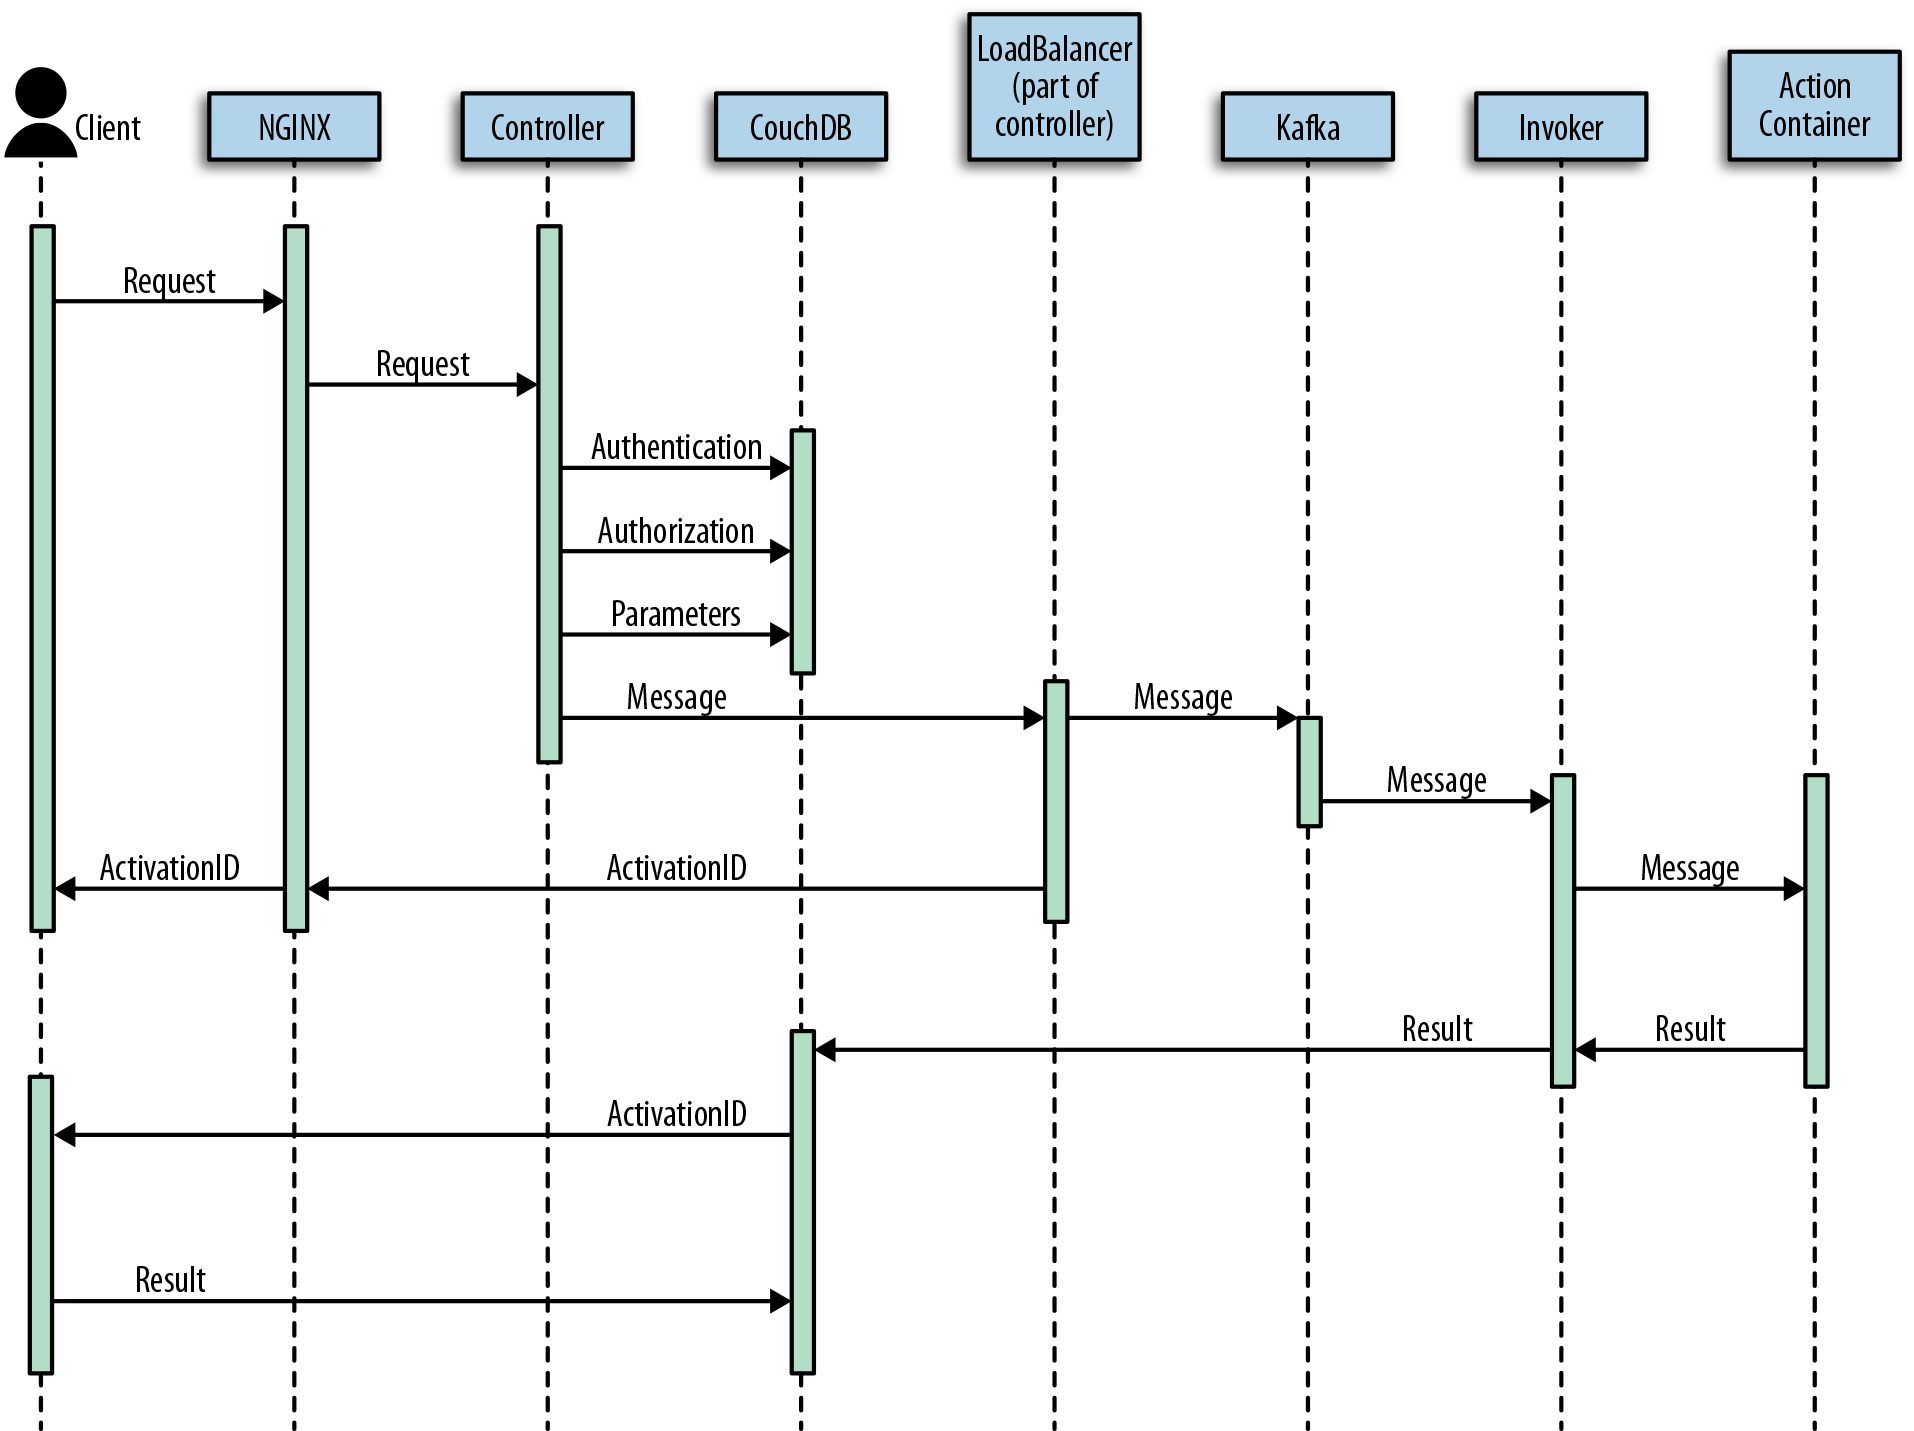
\includegraphics[height=12cm]{Images/action_invokation_timeline}
	\caption{مراحل پردازش \lr{action}}
	\label{تصویر 2-1}
\end{figure}

تمامی‌پردازشی که در \lr{OpenWhisk} انجام می‌شود ناهمگام (\lr{asynchronous}) است. حال با جزئیات بیشتری به بررسی این مراحل می‌پردازیم.

\subsubsection*{\lr{Nginx}}

همه چیز با فراخوانی \lr{action} آغاز می‌شود که این فراخوانی از راه های مختلفی امکان پذیر است:

\begin{itemize}

	\item از طریق وب هنگامی‌که \lr{action} به عنوان \lr{web action} تعریف شده باشد.
	
	\item فراخوانی از \lr{action} دیگر با استفاده از \lr{API}
	
	\item هنگامی‌که یک \lr{trigger} فعال شود و یک \lr{rule} برای فراخوانی \lr{action} وجود داشته باشد.
	
	\item از طریق \lr{CLI}
	
\end{itemize}

\lr{OpenWhisk} یک سیستم \lr{RESTful} است، بنابراین هر فراخوانی \lr{action} به یک درخواست \lr{HTTPS} تبدیل می‌شود و به گره‌ی لبه که همان \lr{Nginx} است می‌رسد. دلیل اصلی وجود وب سرور \lr{Nginx}، پیاده‌سازی و پشتیبانی از پروتکل امن \lr{HTTPS} می‌باشد. \lr{Nginx} پس از دریافت درخواست آن را به سرویس اصلی میانی به نام \lr{Controller} می‌فرستد.

\subsubsection*{\lr{Controller}}

قبل از اجرا شدن \lr{action}، ابتدا \lr{controller} امکان اجرای و صحت آن را بررسی می‌کند. سپس منبع آن هویت سنجی می‌شود تا اجازه دسترسی آن مشخص شود. اگر \lr{action} از دو مرحله قبل عبور کرد، مؤلفه های اضافی به عنوان پیکربندی به آن افزوده می‌شود. حال که امکان اجرای \lr{action} تأیید شد، به قسمت بعدی که \lr{Load Balancer} است فرستاده می‌شود.

\subsubsection*{\lr{Load Balancer}}

وظیفه ی \lr{Load Balancer} همان طور که از نامش پیداست حفظ تعادل میان اجرا کننده های \lr{action} یا همان \lr{invoker} های \lr{OpenWhisk} است. \lr{Load Balancer} با مواظبت از \lr{runtime} های \lr{action} موجود، اگر دوباره مورد نیاز باشد از آن استفاده می‌کند و اگر \lr{runtime} مورد نیاز موجود نبود آن را می‌سازد.

\subsubsection*{\lr{Kafka}}

به جایی رسیدیم که سیستم آماده اجرای \lr{action} است. با این حال، نمی‌توان آن \lr{action} را فوراً به یک \lr{invoker} ارسال کرد، زیرا ممکن است مشغول اجرای یک \lr{action} دیگر باشد. همچنین این احتمال وجود دارد که یک \lr{invoker} خراب شود، یا حتی کل سیستم خراب شده و دوباره راه اندازی شود. بنابراین، از آنجا که ما در یک محیط کاملاً موازی کار می‌کنیم که انتظار می‌رود مقیاس پذیر باشد ، باید این احتمال را در نظر بگیریم که منابع مورد نیاز خود را برای اجرای فوری \lr{action} در دسترس نداشته باشیم. در مواردی از این دست، مجبوریم فراخوانی ها را بافر کنیم. \lr{OpenWhisk} از \lr{Kafka} برای انجام این عمل استفاده می‌کند. \lr{Kafka} یک سیستم پیام رسان "انتشار - اشتراک" با عملکرد بالا است که می‌تواند درخواست ها را تا زمان آماده شدن برای اجرای آن ها ذخیره کند. درخواست که برای ورود به \lr{Nginx} به \lr{HTTPS} تبدیل شده بود، توسط \lr{Load Balancer} به یک پیام \lr{Kafka} تبدیل می‌شود که به \lr{invoker} مقصدش آدرس دهی شده است.

هر پیام ارسال شده به یک \lr{invoker} شناسه ای دارد به نام \lr{activation-ID}. هنگامی‌که پیام در صف \lr{Kafka} قرار می‌گیرد، دو امکان وجود دارد: فراخوانی بدون انسداد و مسدود کننده. برای یک فراخوانی بدون انسداد‌، شناسه فعال سازی به عنوان پاسخ نهایی درخواست به \lr{client} ارسال می‌شود و درخواست تکمیل می‌شود. در این حالت ، پیش بینی می‌شود \lr{client} بعداً برگردد تا نتیجه فراخوانی را بررسی کند. برای یک فراخوانی مسدود کننده، اتصال باز می‌ماند؛ کنترل کننده منتظر نتیجه \lr{action} است و نتیجه را برای سرویس‌گیرنده ارسال می‌کند.

\subsubsection*{\lr{Invoker}}

در \lr{OpenWhisk}، بخش \lr{invoker} وظیفه اجرای \lr{action} را بر عهده دارد. \lr{action} ها در واقع در محیط های جدا شده که توسط کانتیرهای \lr{Docker} ساخته شده اند، اجرا می‌شوند به این صورت که \lr{invoker} ابتدا ایمیج \lr{runtime} مورد نیاز برای اجرای \lr{action} را انتخاب می‌کند و سپس آن را همراه با کد \lr{action} راه اندازی می‌کند.

پس از اینکه \lr{runtime} اجرا شد، \lr{action} هایی که تا آن زمان ساخته و آماده شده اند توسط \lr{invoker} به \lr{runtime} فرستاده می‌شوند. \lr{invoker} همچنین \lr{log} هایی که مربوط به اجرای \lr{action} ها هستند را مدیریت و ذخیره می‌کند.

\subsubsection*{\lr{CouchDB}}

پس از اتمام پردازش، \lr{OpenWhisk} نتیجه را در پایگاه داده \lr{CouchDB} ذخیره می‌کند. سپس تمامی نتایج اجرای \lr{action} ها که در پایگاه داده ذخیره شده‌اند توسط \lr{activation-ID} که به \lr{client} ارسال شده بود، در دسترس هستند.

\subsubsection*{\lr{Client}}

پردازشی که اکنون توضیح داده شد ناهمگام بود. بدان معنی که سرویس‌گیرنده درخواستی را آغاز می‌کند و سپس آن را کنار می‌گذارد، اگرچه آن را به طور کامل فراموش نمی‌کند، زیرا یک شناسه فعال‌سازی را به عنوان نتیجه‌ی فراخوانی دریافت کرده است. همانطور که قبلاً دیدیم، از \lr{activation-ID} برای ذخیره نتیجه در پایگاه داده پس از پردازش استفاده می‌شود. برای بازیابی نتیجه نهایی، سرویس‌گیرنده باید درخواست دیگری را همراه با شناسه فعال سازی به عنوان مؤلفه ورودی ارسال کند. پس از اتمام \lr{action}، نتیجه، \lr{log} ها و سایر اطلاعات در پایگاه داده موجود است و قابل بازیابی است. پردازش همگام هم امکان پذیر است که مانند همان روش پردازش ناهمگام کار می‌کند، اما مسدود کننده است به این معنی که سرویس‌گیرنده منتظر اجرای کامل \lr{action} می‌ماند و نتیجه را فوراً دریافت می‌کند.
